\documentclass[prb,12pt]{revtex4-2}

%font
% Palatino for main text and math
\usepackage[osf,sc]{mathpazo}

% Helvetica for sans serif
% (scaled to match size of Palatino)
\usepackage[scaled=0.90]{helvet}

% Bera Mono for monospaced
% (scaled to match size of Palatino)
\usepackage[scaled=0.85]{beramono}
%actual packages
\usepackage{amsmath, amssymb,physics,amsfonts,amsthm}
\usepackage{enumitem}
\usepackage[most]{tcolorbox}
\usepackage{cancel}
\usepackage{array}
\usepackage{booktabs}
\usepackage{tikz}
\usepackage{hyperref}
\usepackage{enumitem}
\usepackage{transparent}
\usepackage{float}
\usepackage{multirow}
\newtheorem{Theorem}{Theorem}
\newtheorem{Proposition}{Theorem}
\newtheorem{Lemma}[Theorem]{Lemma}
\newtheorem{Corollary}[Theorem]{Corollary}
\newtheorem{Example}[Theorem]{Example}
\newtheorem{Remark}[Theorem]{Remark}
\theoremstyle{definition}
\newtheorem{Problem}{Problem}
\theoremstyle{definition}
\newtheorem{Definition}[Theorem]{Definition}
\newenvironment{parts}{\begin{enumerate}[label=(\alph*)]}{\end{enumerate}}
%tikz
\usepackage{pgfplots}
\usepackage{tikz-3dplot}
\pgfplotsset{compat=1.18}
\usetikzlibrary{patterns}
% definitions of number sets
\newcommand{\N}{\mathbb{N}}
\newcommand{\R}{\mathbb{R}}
\newcommand{\Z}{\mathbb{Z}}
\newcommand{\Q}{\mathbb{Q}}
\newcommand{\C}{\mathbb{C}}
\newcommand*{\circledcirct}{%
	\mathbin{%
		\ooalign{$\circledcirc$\cr\hidewidth$\bullet$\hidewidth}%
	}%
}
\allowdisplaybreaks
\begin{document}
	\title{Lineare Algebra 1 Hausaufgabenblatt Nr. 6}
	\author{Jun Wei Tan}
	\email{jun-wei.tan@stud-mail.uni-wuerzburg.de}
	\affiliation{Julius-Maximilians-Universit\"{a}t W\"{u}rzburg}
	\date{\today}
	\maketitle
%\paragraph{Aufgabe 1.1}
\begin{parts}
	\item 
		\begin{center}
			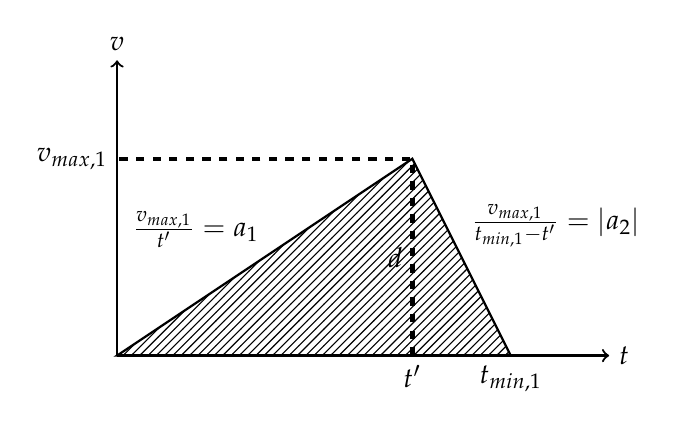
\begin{tikzpicture}[scale=2.5]
				\draw[thick, ->] (0,0) -- (2.5,0);
			\draw[thick, ->] (0,0) -- (0,1.5);
			\filldraw[thick, pattern = north east lines] (0,0) -- (1.5,1) -- (2,0) -- cycle;
			\draw (0,1.5) node[anchor=south] {$v$};
			\draw (2.5,0) node[anchor=west] {$t$};
			\draw (2,0) node[anchor=north] {$t_{min,1}$};
			\draw[ultra thick, dashed] (1.5,0) -- (1.5,1) -- (0,1);
			\draw (0,1) node[anchor=east] {$v_{max,1}$};
			\draw (1.5,0) node[anchor=north] {$t'$};
			\draw (0.4,0.5) node[anchor=south] {$\frac{v_{max,1}}{t'}=a_1$};
			\draw (1.75,0.5) node[anchor=south west] {$\frac{v_{max,1}}{t_{min,1}-t'} = |a_2|$};
			\draw (1.5,0.5) node[anchor=east] {$d$};
			\end{tikzpicture}
		\end{center}
		Man löst die Gleichungen
		\begin{align}
			\frac{1}{2}(v_{max,1})(t_{min,1})=&d\label{eqn1}\\
			v_{max,1}=&a_1t'\label{eqn2}\\
			v_{max,1}=&(t'-t_{min,1})a_2\label{eqn3}
		\end{align}
		Aus \eqref{eqn2} folgt $t'=v_{max,1} / a_1$. Wir setzen das in \eqref{eqn3} ein. Es ergibt sich
		\[
			v_{max,1}=\left( \frac{v_{max,1}}{a_1}-t_{min,1} \right) a_2
		.\] 
		Daraus folgt:
		\[
			v_{max,1}\left( 1-\frac{a_2}{a_1} \right) =-t_{min,1}a_2
		.\] 
	\item 	Noch einmal setzen wir das in \eqref{eqn1} ein:
		\[
			\frac{1}{2}\left[ -t_{min,1}a_2\left( 1-\frac{a_2}{a_1} \right)^{-1} \right] \left( t_{min,1} \right) =d 
		.\] 
		Die L\"{o}sung ist
		\[
			t_{min,1}=\boxed{\left[ -\frac{2d}{a_2}\left( 1-\frac{a_2}{a_1} \right)  \right]^{1 / 2}}
		.\] 
		Aus \eqref{eqn1} folgt
		\[
			v_{max,1}=\frac{2d}{t_{mn,1}}
		.\] 
		Also
		\[
			v_{max,1}=\boxed{\left[ -\frac{1-\frac{a_2}{a_1}}{2a_2d} \right]^{-1 / 2}} 
		.\] 
	\item 
		\begin{center}
			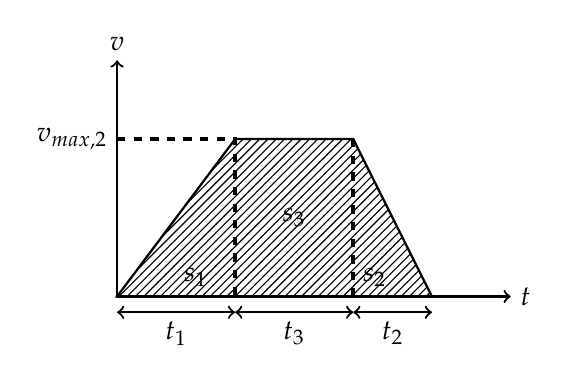
\begin{tikzpicture}[scale=2]
				\draw[thick, ->] (0,0) --(2.5,0);
				\draw[thick, ->] (0,0) -- (0,1.5);
				\filldraw[thick,pattern = north east lines] (0,0) -- (0.75,1) -- (1.5,1) -- (2,0) -- cycle;
				\draw[ultra thick, dashed] (0,1) -- (0.75,1) -- (0.75,0);
				\draw[ultra thick, dashed] (1.5,1) -- (1.5,0);
				\draw (0,1) node[anchor=east] {$v_{max,2}$};
				\draw[thick, <->] (0,-0.1) -- (0.75,-0.1);
				\draw (0.375,-0.1) node[anchor=north] {$t_1$};
				\draw (2.5,0) node[anchor=west] {$t$};
				\draw[thick,<->] (1.5,-0.1) -- (2,-0.1);
				\draw (1.75,-0.1) node[anchor=north] {$t_2$};
				\draw (0,1.5) node[anchor=south] {$v$};
				\draw (0.5,0) node[anchor=south] {$s_1$};
				\draw (1.5,0) node[anchor=south west] {$s_2$};
				\draw (1.125,0.5) node {$s_3$};
				\draw[thick,<->] (0.75,-0.1) -- (1.5,-0.1);
				\draw (1.125,-0.1) node[anchor=north] {$t_3$};
			\end{tikzpicture}
		\end{center}
		Es gilt
		\begin{align*}
			t_1=&\frac{v_{max,2}}{a_1}\\
			t_2=&-\frac{v_{max,2}}{a_2}\\
			s_1=&\frac{1}{2}a_1t_1^2=\frac{v_{max,2}^2}{2a_1}\\
			s_2=&\frac{1}{2}v_{max,2}t_2=-\frac{v_{max,2}^2}{2a_2}\\
			s_3=&v_{max,2}t_3=d-s_1-s_2\\
			t_3=&\frac{d-s_1-s_2}{v_{max,2}}\\
			=&\frac{d}{v_{max,2}}-\frac{v_{max,2}}{2a_1}+\frac{v_{max,2}}{2a_2}\\
			t_{min,2}=&t_1+t_2+t_3\\
			=&\frac{d}{v_{max,2}}+\frac{v_{max,2}}{2a_1}-\frac{v_{max,2}}{2a_2}\\
		\end{align*}

\end{parts}
\paragraph{Aufgabe 1.2}
\begin{center}
	\begin{tikzpicture}[scale=2.5]
		\draw[thick, ->] (0,0) -- (0,{(3-sqrt(3))/(1+sqrt(3))});
		\draw[thick, ->] (0,{(3-sqrt(3))/(1+sqrt(3))}) -- ++({0.4*cos(60)},{0.4*sin(60)});
		\draw (0,{(3-sqrt(3))/(2*(1+sqrt(3)))}) node[anchor=east] {$h_0$};
		\draw[thick, ->] (2,0) -- (2,1);\draw (2,0.5) node[anchor=west] {$h_1$};
		\draw[thick] (0,{(3-sqrt(3))/(1+sqrt(3))}) arc (150:60:{4/(1+sqrt(3))});
		\draw[thick,<->] (0,0) -- (2,0);
		\draw (1,0) node[anchor=north] {$l$};
	\end{tikzpicture}
\end{center}
\begin{gather*}
	x=v_0t\cos\theta\\
	y=v_0t\sin\theta-\frac{1}{2}gt^2\\
	y=x\tan\theta-\frac{gx^2}{2v_0^2\cos^2\theta}
\end{gather*}
Wir brauchen $y(l)=h_1-h_0$, oder
\[
h_1-h_0=l\tan\theta-\frac{gl^2}{2v_0^2\cos^2\theta}
.\] 
Daraus folgt
\[
v_0^2=\frac{gl^2}{2\cos^2\theta\left( l\tan\theta-(h_1-h_0) \right) }
.\] 

\begin{center}
	$l=h_1=1\text{ m},h_0=0\text{ m}$


	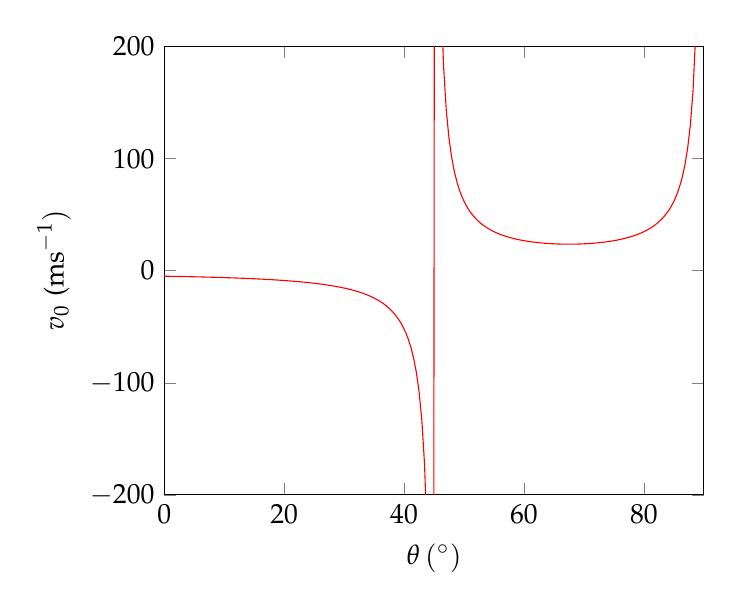
\begin{tikzpicture}
		\begin{axis}[ymin=-200,ymax=200,xmin=0,xmax=90,xlabel=$\theta\left( ^{\circ} \right) $,ylabel=$v_0\text{ (ms}^{-1})$]
\addplot[domain=0:90,color=red,samples=200]{9.81/(2*cos(x)*cos(x)*(tan(x)-1))};
\end{axis}
	\end{tikzpicture}
\end{center}
Es folgt daraus:
\[
y=x\tan\theta-(l\tan\theta-(h_1-h_0))\frac{x^2}{l^2}
.\] 
\paragraph{Aufgabe 1.3}
\begin{center}
	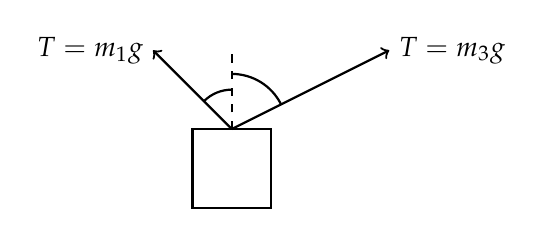
\begin{tikzpicture}
		\draw[thick] (-0.5,-1) rectangle (0.5,0);
		\draw[thick,->] (0,0) -- (-1,1);
		\draw[thick,->] (0,0) -- (2,1);
		\draw[thick, dashed] (0,0) -- (0,1);
		\draw[thick] (0,0.5) arc(90:135:0.5);
		\draw[thick] (0,0.7) arc(90:{atan(0.5)}:0.7);
		\draw (-1,1) node[anchor=east] {$T=m_1g$};
		\draw (2,1) node[anchor=west] {$T=m_3g$};
	\end{tikzpicture}
\end{center}
Es gilt
\begin{align*}
	x:& m_1g\sin\alpha=m_3g\sin\beta\\
	y:& m_1g\cos\alpha+m_3g\cos\beta=m_2g
\end{align*}
Also
\begin{align*}
	m_3=&m_1\frac{\sin\alpha}{\sin\beta}\\
	m_1\cos\alpha+m_1\frac{\sin\alpha}{\sin\beta}\cos\beta=&m_2\\
	m_1=&\frac{m_2}{\cos\alpha+\cos\beta\left( \frac{\sin\alpha}{\sin\beta} \right) }\\
	=& \frac{m_2\sin\beta}{\sin(\alpha+\beta)}\\
	m_3=&\frac{m_2\sin\alpha}{\sin(\alpha+\beta)}
\end{align*}
\begin{center}
	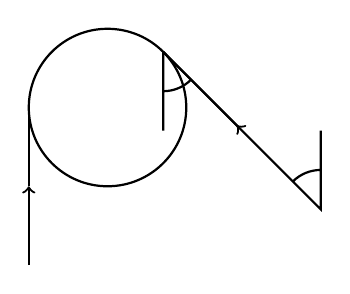
\begin{tikzpicture}
		\draw[thick] (0,0) circle (1);
		\draw[thick,->] (-1,-2) -- (-1,-1);
		\draw[thick] (-1,-1) -- (-1,0);
		\draw[thick,-<] ({1/sqrt(2)},{1/sqrt(2)}) -- ++(1,-1);
		\draw[thick] ({1/sqrt(2)},{1/sqrt(2)}) -- ++(2,-2) -- ++(0,1) -- ++(0,-0.5) arc(90:135:0.5);
		\draw[thick] ({1/sqrt(2)},{1/sqrt(2)}) -- ++(0,-1) -- ++(0,0.5) arc(-90:-45:0.5);
	\end{tikzpicture}
\end{center}
\begin{align*}
	\va F=&-\left[ \begin{pmatrix} 0 \\ -m_1g \end{pmatrix} +m_1g\begin{pmatrix} \sin\alpha \\-\cos\alpha  \end{pmatrix}  \right]\\
	=& m_1g\begin{pmatrix} -\sin\alpha \\ 1+\cos\alpha \end{pmatrix} 
\end{align*}
\paragraph{Aufgabe 1.4}
\begin{parts}
\item 
\noindent \\
	\begin{center}
		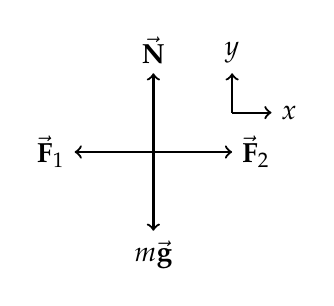
\begin{tikzpicture}
			\draw[thick,->] (0,0) -- (1,0);
			\draw (1,0) node[anchor=west] {$\va F_2$};
			\draw[thick, ->] (0,0) -- (-1,0);
			\draw (-1,0) node[anchor=east] {$\va F_1$};
			\draw[thick,->] (0,0) -- (0,1);
			\draw (0,1) node[anchor=south] {$\va N$};
			\draw (0,-1) node[anchor=north] {$m\va g$};
			\draw[thick, ->] (0,0) -- (0,-1);
			\draw[thick,->]	 (1,0.5) -- (1,1);
			\draw[thick, ->] (1,0.5) -- (1.5,0.5);
			\draw (1,1) node[anchor=south] {$y$};
			\draw (1.5,0.5) node[anchor=west] {$x$};
		\end{tikzpicture}
	\end{center}
\item $a_y=0$ (Zwangsbedingung), $a_x=\frac{1}{3m}\left(|F_2|-|F_1|\right)$
\item \noindent \\
	\begin{center}
		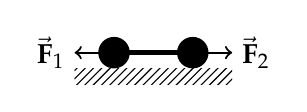
\begin{tikzpicture}[scale=1]
			\fill[pattern = north east lines] (0,-0.2) rectangle (2,0);
		\fill (0.5,0.2) circle (0.2);
	\fill (1.5,0.2) circle (0.2);
	\draw[thick, ->] (0.5,0.2) -- (0,0.2);
	\draw[thick, ->] (1.5,0.2) -- (2,0.2);
	\draw (0,0.2) node[anchor=east] {$\va F_1$};
	\draw (2,0.2) node[anchor=west] {$\va F_2$};
	\draw[ultra thick] (0.5,0.2) -- (1.5,0.2);
		\end{tikzpicture}
	\end{center}
	\[
	a_1=a_2=\frac{1}{3m}\left(|\va F_2|-|\va F_1| \right) 
	.\] 
\item \noindent \\
	\begin{center}
		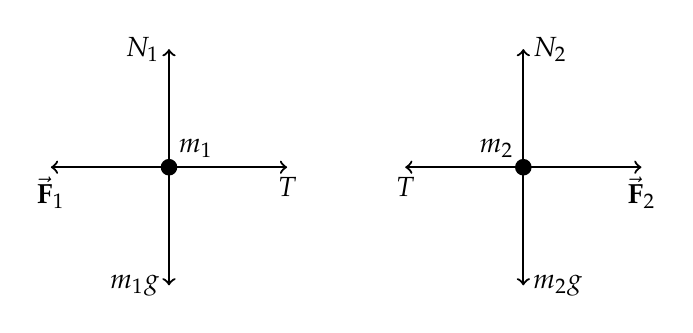
\begin{tikzpicture}[scale=1.5]
		\fill (0,0) circle (2pt);
		\draw[thick, ->] (0,0) -- (1,0);
		\draw[thick, ->] (0,0) -- (0,1);
		\draw[thick, ->] (0,0) -- (-1,0);
		\draw[thick, ->] (0,0) -- (0,-1);
	\fill (3,0) circle (2pt);
	\draw[thick, ->] (3,0) -- (4,0);
	\draw[thick, ->] (3,0) -- (3,1);
	\draw[thick, ->] (3,0) -- (3,-1); 
	\draw[thick, ->] (3,0) -- (2,0);
	\draw (1,0) node[anchor=north] {$T$};
	\draw (0,1) node[anchor=east] {$N_1$};
	\draw (0,-1) node[anchor=east] {$m_1g$};
	\draw (-1,0) node[anchor=north] {$\va F_1$};
	\draw (4,0) node[anchor=north] {$\va F_2$};
	\draw (2,0) node[anchor=north] {$T$};
	\draw (3,1) node[anchor=west] {$N_2$};
	\draw (3,-1) node[anchor=west] {$m_2g$};
	\draw (0,0) node[anchor=south west] {$m_1$};
	\draw (3,0) node[anchor=south east] {$m_2$};
		\end{tikzpicture}
	\end{center}
\item 
	\begin{align*}
		m_1a=&T-F_1\\
		m_2a=& F_2-T\\
		(m_1+m_2)a=&T-F_1+F_2-T\\
		=&F_2-F_1\\
		=&3ma\\
		a=&\frac{1}{3m}\left( F_2-F_1 \right) 
	\end{align*}
\end{parts}

%\begin{Problem}
	Es seien die Punkte $x_0, x_1, \dots, x_n$ mit $x_i \in \R$ gegeben. Wir definieren den Operator
	\[
		\Phi:\R_{\le n}[x]\to \R^{n+1}, p\to y, \text{ mit }p(x_i)=y_i, i=0,\dots,n
	\] 
	wobei wir mit $\R_{\le n}[x]$ den Raum der Polynome mit reellen Koeffizienten vom Grad höchsten $n$ bezeichnen und $p(x)$ die Auswertung des Polynoms $p$ im Punkt $x$ beschreibt.
	\begin{parts}
		\item  Zeigen Sie: Sind die Punkte $x_i$ paarweise verschieden, so ist die Abbildung $\Phi$ wohldefiniert und isomorph. (Eine Konsequenz hieraus ist die eindeutige Lösbarkeit der Polynominterpolation.)
		\item Was passiert, wenn Sie nicht fordern, dass die $x_i$ paarweise verschieden sind? Kann $\Phi$ im Allgemeinen noch injektiv (surjektiv) sein?
	\end{parts}
\end{Problem}
\begin{proof}
	\begin{parts}
\item Injektiv: Nehme an, dass es zwei unterschiedliche Polynome $p_1$, $p_2$ gibt, mit $p_1(x_i)=p_2(x_i)\forall i=0,\dots,n$. Dann ist $p(x):=p_1(x)-p_2(x)$ auch ein Polynom, mit $p(x_i):=0\forall i\in \{0,\dots,n\}$. Weil  $ \deg(p)\le n$ist, folgt daraus, dass $\forall x,p(x)=0, p_1(x)=p_2(x)$. Das ist ein Widerspruch.

	Surjektive: Sei $(y_0,\dots,y_n)\in \R^{n+1}$. Dann ist
	\[
	p(x)=(x-y_0)(x-y_1)\dots(x-y_n)
	\]
	auch ein Polynom mit $\Phi(p)=(y_0,\dots,y_n)$.

	Linearität: Sei $p_1(x),p_2(x)\in \R_{\le n}[x], a\in \R$. Sei auch $p(x)=p_1(x)+p_2(x)$. Es gilt dann
	\[
	p(x_i)=p_1(x_i)+p_2(x_i),i=0,\dots,n\] und daher
	\[
	\Phi(p)=\Phi(p_1+p_2)=\Phi(p_1)+\Phi(p_2)
	.\] 
	Es gilt auch, f\"{u}r $p(x):=ap_1(x)$, dass
	\[
	p(x_i)=ap_1(x_i), i=0,\dots,n
	,\]
	und daher
	\[
	\Phi(p)=\Phi(ap_1)=a\Phi(p_1)
	.\] 
\item Nein. Sei, zum Beispiel, $n=1$, $x_0=x_1=0$. Dann gilt
	\begin{align*}
		\Phi(x)=&(0,0)^T\\
		\Phi(x^2)=&(0,0)^T
	\end{align*}
	Aber die zwei Polynome sind ungleich.
	\end{parts}
\end{proof}

\begin{Problem}
	\begin{parts}	
	\item Es sei eine Matrix $A \in \mathbb{K}^{n\times n}$ gegeben. Wir bilden die erweiterte Matrix
	\[
		B=(A|1_n)\]
		mit $1_n$ die Einheitsmatrix in $\R^n$. Zeigen Sie: $A$ ist genau dann invertierbar, wenn $A$ durch elementare Zeilenumformung in die Einheitsmatrix überführt werden kann. Verfizieren Sie weiterhin: Werden die dafür benötigten Zeilenumformungen auf ganz $B$ angewendet, so ergibt sich im hinteren Teil, wo zu Beginn die Einheitsmatrix stand, genau $A^{-1}$.
	\item Es sei nun
		\[
			A=\begin{pmatrix} 1 & 0 & 0 & 1\\0 & -1 & 2 & 0 \\ 0 & 0 & 0 & -2\\3 & 0 & 1 & 2 \end{pmatrix} 
		.\] 
		Bestimmen Sie $A^{-1}$.
	\end{parts}
\end{Problem}
\begin{proof}
	\begin{parts}
	\item Definiert $(x,y),x\in \mathbb{K}^n,y\in\mathbb{K}^m$ durch $\mathbb{K}^{n+m}\ni(x,y)=(x_1,\dots,x_n,y_1,\dots,y_n)$. Eine solche erweiterte Matrix bedeutet eine Gleichungssystem durch
		\[
		B(x, -y)=Ax-1_ny=0
		,\]
		wobei $x,y\in \mathbb{K}^n$. F\"{u}r jeder $x\in\mathbb{K}^n$ gibt es $y\in \mathbb{K}^n,$ so dass $B(x,-y)=0$. Nehme an, dass wir durch elementare Zeilenumformung
		\[
		B=(A|1_n)\to (1_n, A'):=B'
		\]
		kann. Die Gleichungssystem ist dann $x=A'y$. Dadurch können wir f\"{u}r jeder  $y\in\mathbb{K}^n$ eine $A'y=x\in\mathbb{K}^n$ rechnen, f\"{u}r die gilt, dass $Ax=y$. Das heißt, dass $A'=A^{-1}$. 
	\item
		{\allowdisplaybreaks
		\begin{gather*}
			\left(
\begin{array}{cccc|cccc}
 1 & 0 & 0 & 1 & 1 & 0 & 0 & 0 \\
 0 & -1 & 2 & 0 & 0 & 1 & 0 & 0 \\
 0 & 0 & 0 & -2 & 0 & 0 & 1 & 0 \\
 3 & 0 & 1 & 2 & 0 & 0 & 0 & 1 \\
\end{array}
\right) \xrightarrow{R_4-3R_1} \left(
\begin{array}{cccc|cccc}
 1 & 0 & 0 & 1 & 1 & 0 & 0 & 0 \\
 0 & -1 & 2 & 0 & 0 & 1 & 0 & 0 \\
 0 & 0 & 0 & -2 & 0 & 0 & 1 & 0 \\
 0 & 0 & 1 & -1 & -3 & 0 & 0 & 1 \\
\end{array}
\right) \xrightarrow{R_2\times -1}\\ \left(
\begin{array}{cccc|cccc}
 1 & 0 & 0 & 1 & 1 & 0 & 0 & 0 \\
 0 & 1 & -2 & 0 & 0 & -1 & 0 & 0 \\
 0 & 0 & 0 & -2 & 0 & 0 & 1 & 0 \\
 0 & 0 & 1 & -1 & -3 & 0 & 0 & 1 \\
\end{array}
\right) \xrightarrow{R_3\leftrightarrow R_4} \left(
\begin{array}{cccc|cccc}
 1 & 0 & 0 & 1 & 1 & 0 & 0 & 0 \\
 0 & 1 & -2 & 0 & 0 & -1 & 0 & 0 \\
 0 & 0 & 1 & -1 & -3 & 0 & 0 & 1 \\
 0 & 0 & 0 & -2 & 0 & 0 & 1 & 0 \\
\end{array}
\right) \xrightarrow{R_2+2R_3}\\ \left(
\begin{array}{cccc|cccc}
 1 & 0 & 0 & 1 & 1 & 0 & 0 & 0 \\
 0 & 1 & 0 & -2 & -6 & -1 & 0 & 2 \\
 0 & 0 & 1 & -1 & -3 & 0 & 0 & 1 \\
 0 & 0 & 0 & -2 & 0 & 0 & 1 & 0 \\
\end{array}
\right) \xrightarrow{R_2-R_4} \left(
\begin{array}{cccc|cccc}
 1 & 0 & 0 & 1 & 1 & 0 & 0 & 0 \\
 0 & 1 & 0 & 0 & -6 & -1 & -1 & 2 \\
 0 & 0 & 1 & -1 & -3 & 0 & 0 & 1 \\
 0 & 0 & 0 & -2 & 0 & 0 & 1 & 0 \\
\end{array}
\right) \xrightarrow{R_4\times -\frac{1}{2}}\\ \left(
\begin{array}{cccc|cccc}
 1 & 0 & 0 & 1 & 1 & 0 & 0 & 0 \\
 0 & 1 & 0 & 0 & -6 & -1 & -1 & 2 \\
 0 & 0 & 1 & -1 & -3 & 0 & 0 & 1 \\
 0 & 0 & 0 & 1 & 0 & 0 & -\frac{1}{2} & 0 \\
\end{array}
\right) \xrightarrow{R_1-R_4} \left(
\begin{array}{cccc|cccc}
 1 & 0 & 0 & 0 & 1 & 0 & \frac{1}{2} & 0 \\
 0 & 1 & 0 & 0 & -6 & -1 & -1 & 2 \\
 0 & 0 & 1 & -1 & -3 & 0 & 0 & 1 \\
 0 & 0 & 0 & 1 & 0 & 0 & -\frac{1}{2} & 0 \\
\end{array}
\right) \xrightarrow{R_3+R_4} \\\left(
\begin{array}{cccc|cccc}
 1 & 0 & 0 & 0 & 1 & 0 & \frac{1}{2} & 0 \\
 0 & 1 & 0 & 0 & -6 & -1 & -1 & 2 \\
 0 & 0 & 1 & 0 & -3 & 0 & -\frac{1}{2} & 1 \\
 0 & 0 & 0 & 1 & 0 & 0 & -\frac{1}{2} & 0 \\
\end{array}
\right)
		\end{gather*}
	}
	\end{parts}
\end{proof}
\begin{Problem}
	Es seien die Vektorräume $V, W$ über $\mathbb{K}$ gegeben mit $\dim(V) = n$ und $\dim(W ) = m$. Wir betrachten eine lineare Abbildung
	\[
	T:V\to W, v\to T(v)\] 
Seien $B_V$ und $B_W$ Basen von $V$, bzw. $W$. Wir nehmen an $T$ ist nicht die konstante Nullabbildung. Beweisen Sie:
\begin{parts}
\item Der Kern von $_{B_W}[T]_{B_V}$ ist entweder trivial (d.h. nur die 0) oder hängt nur von der Wahl von $B_V$ ab, aber nicht von $B_W$.
\item Das Bild von $_{B_W}[T]_{B_V}$ ist entweder der ganze $\mathbb{K}^m$ oder hängt nur von der Wahl von $B_W$ ab, aber nicht von $B_v$. 
\item Der Rang von $_{B_W}[T]_{B_V}$ ist unabh\"{a}ngig von $B_w$ und $B_V$.
aber nicht von $B_W$.
\end{parts}
\end{Problem}
\begin{proof}
Nach Korollar 5.43 gilt, f\"{u}r $A,A' \subseteq V$ und $B,B'\subseteq W$ Basen der Vektorräume $V$ und $W$ über $\mathbb{K}$, und $\Phi\in \text{Hom}(V,W)$.
 \[
	 _{B'}\left[ \Phi \right]_{A'}={}_{B'}[\text{id}_W]_B\cdot{}_B[\Phi]_A\cdot{}_A[\text{id}_V]_{A'}
.\] 
\begin{Lemma}
	Jeder Basiswechsel f\"{u}r sowohl $B_V$ als auch $B_W$ kann als zwei Basiswechseln interpretiert werden, wobei eine Basiswechsel nur $B_V$ verändert, und die andere nur $B_W$.
\end{Lemma}
\begin{proof}
	\[
		_{B'}\left[ \Phi \right]_{A'}={}_{B'}[\text{id}_W]_B\cdot{}_B[\Phi]_A\cdot{}_A[\text{id}_V]_{A'}={}_{B'}[\text{id}_W]_B\left( {}_B[\text{id}_W]_B\cdot {}_B[\Phi]_A\cdot {}_A[\text{id}]_{A'} \right) {}_A[\text{id}_V]_A
	.\]
	(In den Klammern gibt es zuerst ein Basiswechsel in $V$, dann ein Basiswechsel in $W$ ). Ein ähnliche Argument zeigt, dass wir zuerst ein Basiswechseln in $W$ betrachten kann.
\end{proof}
\begin{Corollary}
	In jedem Teilaufgabe muss man nur das Fall betrachten, in dem entweder $B_V$ oder $B_W$ sich verändert. 
\end{Corollary}
	\begin{parts}
	\item 
	\end{parts}
\end{proof}

%\begin{Problem}
	\begin{parts}
		\item  Berechnen Sie alle möglichen Matrixprodukte der folgenden Matrizen. Was muss jeweils für die Dimensionen erfüllt sein?
	 \begin{gather*}
		 A=\begin{pmatrix} 1 & -1 & 2 \\ 0 & 3 & 5 \\ 1 & 8 & 7 \end{pmatrix}, B=\begin{pmatrix} -1 & 0 & 1 & 0 \\ 0 & 1 & 0 & -1 \\ 1 & 0 & -1 & 0 \end{pmatrix} ,C=\begin{pmatrix} 1 \\ 0 \\ 8 \\ -7 \end{pmatrix}\\
		 D=\begin{pmatrix} -1 & 2 & 0 & 8 \end{pmatrix}, E=\begin{pmatrix} 1 & 4 \\ 0 & 5 \\ 6 & 8 \end{pmatrix} , F=\begin{pmatrix} -1 & 2 & 0 \end{pmatrix} .
	 \end{gather*}
 \item Eine Blockmatrix ist eine Matrix von der Form
	 \[
		 A=\begin{pmatrix} A_1 & A_3 \\ A_2 & A_4 \end{pmatrix} \] 
		 mit Matrizen $A_1\in \mathbb{K}^{n \times m}, A_2\in \mathbb{K}^{n'\times m}, A_3\in \mathbb{K}^{n \times m'}, A_4\in\mathbb{K}^{n'\times m'}$. Sei weiterhin
		 \[
			 B=\begin{pmatrix} B_1 & B_3 \\ B_2 & B_4 \end{pmatrix} \] 
			 mit ebenso Einträgen aus $\mathbb{K}$. Wer nun meint, die Multiplikation von A und B sei so simpel wie
			 \[
				 A\cdot B=\begin{pmatrix} A_1B_1+A_3B_2 & A_1B_3+A_3B_4 \\ A_2B_1+A_4B_2 & A_2B_3+A_4B_4 \end{pmatrix} \] 
hat tatsächlich recht. Beweisen Sie diese Formel und geben Sie gleichzeitig die $B_i'$s für die benötigten Matrizenräume an, sodass die Rechnung wohldefiniert ist.
 \end{parts}
\end{Problem}
\begin{proof}
	\begin{parts}
	\item F\"{u}r $A$ eine $n\times m$ Matrize, und $B$ eine $p\times q$ Matrize, ist $AB$ wohldefiniert, nur wenn $m=p$

		Die Matrizprodukte sind
		\begin{gather*}
			AB=\begin{pmatrix} 1 & -1 & -1 & 1\\5 & 3 & -5 & -3 \\ 6 & 8 & -6 & -8 \end{pmatrix}\\
			AE=\begin{pmatrix} 13 & 15 \\ 30 & 55 \\ 43 & 100 \end{pmatrix} \\
			FA=\begin{pmatrix} -1 & 7 & 8 \end{pmatrix}\\ 
			BC=\begin{pmatrix} 7 \\ -7 \\ -7 \end{pmatrix}\\
			CD=\begin{pmatrix} -1 & 2 & 0 & 8 \\ 0 & 0 & 0 & 0\\-8 & 16 & 0 & 64\\-7 & 14 & 0 & 56 \end{pmatrix}\\
			DC=(55)\\
			CF=\begin{pmatrix} -1 & 2 & 0 \\ 0 & 0 & 0 \\ -8 & 16 & 0\\-7 & 14 & 0 \end{pmatrix}\\ 
			FE=\begin{pmatrix} -1 & 6 \end{pmatrix} 
		\end{gather*}
	\item Wir brauchen $B_1\in\mathbb{K}^{m\times p},B_2\in\mathbb{K}^{m'\times p}, B_3\in\mathbb{K}^{m\times q}, B_4\in\mathbb{K}^{m'\times q}$ f\"{u}r $p,q\in \N$. Wir bezeichnen, f\"{u}r $v_1\in\mathbb{K}^a,v_2\in\mathbb{K}^b$, das Vektor $(v_1,v_2)\in\mathbb{K}^{a+b}$. Sei jetzt $v_1\in \mathbb{K}^p,v_2\in\mathbb{K}^q$.
		{\allowdisplaybreaks
		\begin{align*}
			AB(v_1,v_2)=&A\begin{pmatrix} B_1 & B_3 \\ B_2 & B_3 \end{pmatrix}\begin{pmatrix} v_1 \\ v_2 \end{pmatrix} \\ 
			=&A\begin{pmatrix} \smash{\overbrace{B_1v_1+B_3v_2}^{\in\mathbb{K}^m}}\vphantom{B_1v_1}\\ \smash{\underbrace{B_2v_1+B_4v_2}_{\in\mathbb{K}^n}}\vphantom{B_1v_1} \end{pmatrix} \vphantom{\begin{pmatrix} \overbrace{B_1v_1}^{\in \mathbb{K}^a}\\ \underbrace{B_1V_1}_{\in\mathbb{K}^a} \end{pmatrix} } \\
			=&\begin{pmatrix} A_1 & A_3 \\ A_2 & A_4 \end{pmatrix}\begin{pmatrix} B_1v_1+B_3v_2\\B_2v_1+B_4v_2 \end{pmatrix} \\
			=&\begin{pmatrix} A_1(B_1v_1+B_3v_2)+A_3(B_2v_1+B_4v_2)\\ A_2(B_1v_1+B_3v_2)+A_4(B_2v_1+B_4v_2) \end{pmatrix}\\
			=&\begin{pmatrix} A_1B_1+A_3B_2 & A_1B_3+A_3B_4 \\ A_2B_1+A_4B_2 & A_2B_3+A_4B_4 \end{pmatrix} \begin{pmatrix} v_1 \\ v_2 \end{pmatrix} \qedhere
		\end{align*}
	}
	\end{parts}
\end{proof}
\begin{Problem}
	Es seien $V$ und $W$ Vektorräume über K, nicht notwendigerweise endlich-dimensional und
	\[
	\Phi:V\to W
	\]
	eine lineare Abbildung. Beweisen Sie:
	\begin{parts}
	\item Die duale Abbildung $\Phi^*$ ist injektiv genau dann, wenn $\Phi$ surjektiv ist.
		{\footnotesize Hinweis: Die Richtung $\implies$ beweisen Sie am einfachsten als eine Kontraposition.}
	\item Die duale Abbildung $\Phi^*$ ist surjektiv genau dann, wenn $\Phi$ injektiv ist.
		{\footnotesize Hinweis: Die Rückrichtung lässt sich am einfachsten direkt beweisen. Nutzen Sie in dem Fall die Injektivität von $\Phi$ aus, um f\"{u}r ein beliebiges $v^*\in V^*$ eine lineare Abbildung im Bild von $\Phi^*$ zu konstruieren, die die gleichen Werde wie Abbildung $v^*$ liefert.}
	\item Im Falle der Invertierbarkeit gilt
		\[
			\left( \Phi^{-1} \right) ^*=\left( \Phi^* \right) ^{-1}
		.\] 
	\end{parts}
\end{Problem}
\begin{proof}
	\begin{parts}
	\item Sei $\Phi$ surjektiv, und $w_1^*,w_2^*\in W^*$. Es gilt $\Phi w_1^*=w_1^*\circ \Phi, \Phi w_2^*=w_2^*\circ \Phi$. Die zwei Abbildungen  $w_1^*\circ \Phi$ und $w_2^*\circ \Phi$ sind unterschiedliche, solange es mindestens ein $v\in V$ gibt, sodass $(w_1^*\circ\Phi)(v)\neq (w_2^*\circ\Phi)(v)$. Wir haben aber ausgenommen, dass $w_1^*\neq w_2^*$. Das bedeutet, dass es $w\in W$ gibt, so dass $w_1^*(w)\neq w_2^*(w)$. Weil $\Phi$ surjektiv ist, ist $w=\Phi(v)$ f\"{u}r eine $v$. Dann ist $(w_1^*\circ\Phi)(v)\neq (w_2^*\circ\Phi)(v)$, also  $\Phi^*$ ist injektiv.

		Jetzt nehmen wir an, dass $\Phi$ nicht surjektiv ist, also es gibt ein Unterraum $U\subseteq W$, sodass $U\backslash \left\{ 0 \right\} \cap \text{im}(\Phi)=\varnothing$. Dann können wir zwei lineare Abbildungen $w_1^*$ und $w_2^*$ definieren, die auf $\text{im}(\Phi)$ gleich sind, aber auf $U$ ungleich sind. Es gillt $\Phi^*(w_1)=\Phi^*(w_2)$, aber $w_1\neq w_2$, also $\Phi^*$ ist nicht injektiv. 
	\item Zuerst beweisen wir: $\Phi$ nicht injektiv $\implies$ $\Phi^*$ nicht surjektiv.
		Sei $v_1,v_2\in V,v_1\neq v_2$ und $\Phi(v_1)=\Phi(v_2)=w$.Es gibt eine lineare Abbildung $v^*\in V^*$, so dass $v^*(v_1)\neq v^*(v_2)$. Sei aber $w^*\in W^*$. Es gilt $\left( \Phi^* w^* \right)(v) =(w^*\circ\Phi)(v)$. Dann ist
		\[
		\Phi^*w^*(v_1)=\Phi^*(w)=\Phi^*w^*(v_2)
		,\] 
		also $\Phi^*(w^*)\neq v^*$ f\"{u}r alle $w^*\in W^*$. Es folgt: $\Phi^*$ ist nicht surjektiv.

		Jetzt beweisen wir $\Phi$ injektiv $\implies$ $\Phi^*$ surjektiv. Sei $v^*\in V^*$. Wir definieren eine Abbildung (momentan nicht unbedingt linear) so: F\"{u}r alle  $w\in \text{im}(\Phi)$, also  $w=\Phi(v)$, ist $w^*(w)=v^*(v)$. F\"{u}r  $w\not\in \text{im}(\Phi)$ ist $w^*(w)=0$. 

		Es ist klar, dass $w^*\circ \Phi=v^*$. Wir müssen nur zeigen, dass $w^*$ linear ist, also $w^*\in W^*$.
		 \begin{enumerate}[label=(\arabic*)]
			 \item Sei $w\in W$, $a\in \mathbb{K}$. Falls $w \not\in \text{im}(\Phi)$, ist auch $aw\not\in \text{im}(\Phi)$. Es gilt daher
				 \[
				 w^*(aw)=aw^*(w)=0
				 .\] 
				 Falls $w\in \text{im}(\Phi)$, also $w=\Phi v$ f\"{u}r ein $v\in V$, gilt auch $aw=\Phi(av)$, und
				 \[
				 w^*(aw)=v^*(av)=av^*(v)=aw^*(w)
				 .\] 
		\end{enumerate}
		Daraus folgt: $w^*\in W^*$, und $\Phi^*(w^*)=v^*$.
	\item In den letzten Teilaufgaben haben wir bewiesen, dass wenn $\Phi$ bijektiv ist, ist $\Phi^*$ auch bijektiv. Die Rückrichtung stimmt auch. Wir müssen nur Gleichheit zeigen.

		\begin{tcolorbox}[title=Vereinfachung]
Wir müssen nur zeigen, per Definition eine Inverseabbildung, dass
			\[
				\Phi^*\circ \left( \Phi^{-1} \right) ^*=\text{id}_{V^*}
			.\] 
			(Wir müssen nicht zeigen, dass $\left( \Phi^{-1} \right) ^*\circ\Phi^*=\text{id}_W$, weil die beide Abbildungen bijektiv sind.)
		\end{tcolorbox}
		Es gilt, f\"{u}r $v^*\in V^*$, $\left( \Phi^{-1} \right)^*(v^*)=v^*\circ\Phi^{-1}$. Daraus folgt
		\begin{align*}
			\left(\Phi^*\circ\left( \Phi^{-1} \right)^*\right)(v^*)=&\Phi^*\left( v^*\circ \Phi^{-1} \right) \\
			=& v^*\circ\Phi^{-1}\circ\Phi\\
			=& v^*\qedhere
		\end{align*}
	\end{parts}
\end{proof}
\begin{Problem}	\textbf{(Darstellung eines Unterraums)}
	\begin{parts}
\item Es sei $A\in\mathbb{K}^{n\times m}$. Beweisen Sie: Das Gleichungssystem $Ax=b$ hat genau dann eine Lösung in $x\in \mathbb{K}^m$, wenn f\"{u}r alle $y\in \mathbb{K}^m$ aus  $A^Ty=0$ folgt $b^Ty=0$.
\item Es sei
	\[
		U=\text{span}\left\{ \begin{pmatrix} 1 \\ 1 \\ 1 \\ 1 \end{pmatrix} ,\begin{pmatrix} 1 \\ 1 \\ -1 \\ -1 \end{pmatrix}  \right\} \subset \R^4
	.\] 
\item Verwenden Sie (a) um eine Matrix $B$ zu konstruieren, sodass gilt
	\[
		U=\text{ker}(B)
	.\] 
\end{parts}
\end{Problem}
\begin{proof}
\begin{parts}
\item 
	\begin{enumerate}
		\item Sei $x$ eine Lösung, $Ax=b$, und $y\in \mathbb{K}^m$ beliebig, sodass $A^Ty=0$. Es gilt dann:
			 \[
			x^TA^Ty=b^Ty=0
			.\] 
	\end{enumerate}
\item Wir machen eine Basisergänzung:
	\[
		\R^4=\text{span}\left\{ \begin{pmatrix} 1 \\ 1 \\ 1 \\ 1 \end{pmatrix},\begin{pmatrix} 1 \\ 1 \\ -1 \\ -1 \end{pmatrix}, \begin{pmatrix} 0 \\ 1 \\ 0 \\ 0 \end{pmatrix}, \begin{pmatrix} 0 \\ 0 \\ 1 \\ 0 \end{pmatrix}  \right\} 
	.\] 
Sei 
\[
	A=\begin{pmatrix} 1 & 1 & 0 & 0\\1 & 1 & 1 & 0 \\ 1 & -1 & 0 & 1 \\ 1 & -1 & 0 & 0 \end{pmatrix} 
.\] 
Wir brauchen $B\in\mathbb{R}^{4\times 4}$, sodass
\[
	BA=\begin{pmatrix} 0 & 0 & w_{1,1} & w_{2,1}\\ 0 & 0 & w_{1,2} & w_{2,2} \\ 0 & 0 & w_{1,3} & w_{2,3} \\ 0 & 0 & w_{1,4} & w_{2,4} \end{pmatrix}:=C 
,\] 
wobei $(w_{1,1}, w_{1,2}, w_{1,3}, w_{1,4})^T$ und $(w_{2,1},w_{2,2},w_{2,3},w_{2,4})^T$ linear unabhängig sind, also $B=CA^{-1}$. Weil
 \[
	 A^{-1}=\begin{pmatrix} \frac{1}{2}& 0 & 0 & \frac{1}{2}\\ \frac{1}{2}& 0 & 0 & -\frac{1}{2}\\ -1 & 1 & 0 & 0 \\ 0 & 0 & 1 & -1 \end{pmatrix} 
,\] 
Wir nehmen außerdem 
\[
	C=\begin{pmatrix}  0 & 0 & 1 & 0 \\ 0 & 0 & 0 & 1\\ 0 & 0 & 0 & 0 \\ 0 & 0 & 0 & 0 \end{pmatrix} 
,\] 
also
\[
	B=\begin{pmatrix} -1 & 1 & 0 & 0\\0 & 0 &1 & -1\\ 0 & 0 & 0 & 0 \\ 0 & 0 & 0 & 0 \end{pmatrix} 
.\qedhere\] 
\end{parts}
\end{proof}

%	\begin{Problem}\label{pr:linalg1-4.1}
	Direktes Produkt
	\begin{parts}
		\item Zeigen Sie: Sind $(G,*,e_G)$ und $(H,\star, e_H)$ Gruppen, dann ist auch $G\times H$ mit der Verknüpfung
			\[
			\odot\left( G\times H \right) \times \left( G\times H \right) \to G\times H, \qquad (g_1,h_1)\odot(g_2,h_2):=(g_1*g_2,h_1\star h_2)
			\] 
			und dem neutralen Element $(e_G,e_H)$ eine Gruppe. Diese Gruppe nennt man auch das \emph{direktes Produkt} von $G$ und $H$.
		\item Zeigen Sie: Sind $(R,+,\cdot)$ und $(S,\star,*)$ Ringe, dann ist auch $R\times S$ mit den Verkn\"{u}pfung $\oplus$ und $\odot$, definiert durch $(r_1,s_1)\oplus (r_2,s_2):=(r_1+r_2,s_1\star s_2)$ bzw. $(r_1,s_1)\odot (r_2,s_2):= (r_1\cdot r_2, s_1* s_2)$ ein Ring.
		\item Beweisen oder widerlegen Sie: Ist $(K,+,\cdot)$ ein Körper, dann ist auch $K \times K$ mit den Verknüpfungen wie in (b) ein Körper.
	\end{parts}
\end{Problem}
\begin{proof}
	\begin{parts}
	\item 
		\begin{enumerate}[label=(\roman*)]
			\item (Assoziativität) 
\begin{align*}
	(g_1,h_1)\odot ((g_2,h_2)\odot(g_3,h_3))=&(g_1,h_1)\odot(g_2*g_3,h_2\star h_3)\\
	=& (g_1*(g_2*g_3), h_1\star(h_2\star h_3))\\
	=& ((g_1*g_2)*g_3,(h_1\star h_2)\star h_3)\\ 
	=& (g_1*g_2,h_1\star h_2)\odot (g_3,h_3)\\
	=& ((g_1,h_1)\odot (h_1,h_2))\odot (g_3,h_3)
\end{align*}
\item (Neutrales Element)
	\[
		(g_1,h_1)\odot (e_G,e_H)=(g_1,h_1)=(e_G,e_H)\odot (g_1,h_1)
	.\] 
\item (Existenz des Inverses) Sei $(g_1,h_1)\in G\times H$. Weil $G$ und $H$ gruppe sind, gibt es elemente $g_1^{-1}\in G, h_1^{-1}\in H$, sodass $g_1*g_1^{-1}=e_G=g_1^{-1}*g_1$ und $h_1\star h_1^{-1}=e_H=h_1^{-1}\star h_1$. Es gilt
	\[
		(g_1,h_1)\odot(g_1^{-1},h_1^{-1})=(g_1*g_1^{-1},h_1\star h_1^{-1})=(e_G,e_H)
	,\]
	und ähnlich auch $(g_1^{-1},h_1^{-1})\odot (g_1,h_1)=(e_G,e_H)$
		\end{enumerate}
		Schluss: $ (G\times H, \odot, (e_G,e_H))$ ist eine Gruppe.
	\item 
		\begin{enumerate}[label=(\roman*)]
			\item $(R\times S,\oplus, (0_R, 0_S))$ ist eine abelsche Gruppe.

				Folgt aus (a).
\item $\oplus$ ist assoziativ:

	Beweis läuft ähnlich zu (a), die Behauptung folgt aus die Assoziativität von $\cdot$ und $*$.
\item Distributivgesetz:
	 \begin{align*}
		 (r_1,s_1)\odot\left( (r_2,s_2)\oplus(r_3,s_3) \right) =& (r_1,s_1)\odot(r_2+r_3,s_2\star s_3)\\
		 =&(r_1\cdot (r_2+r_3),s_1*(s_2\star s_3))\\
		 =&(r_1\cdot r_2+r_1\cdot r_3, s_1*s_2\star s_1*s_3)\\
		 =&(r_1\cdot r_2, s_1*s_2)\oplus (r_1\cdot r_3, s_1*s_3)\\
		 =&\left[(r_1,s_1)\odot(r_2,s_2)\right]\oplus \left[ (r_1,s_1)\odot (r_3,s_3) \right] 
	\end{align*}
		\end{enumerate}
	\item Falsch. Sei $x,y\in K$ beliebige Elemente von $K$. Es ist klar, dass $(0,0)$ das Nullelement ist, weil
		\[
			(x,y)\oplus(0,0)=(x+0,y+0)=(x,y)
		.\] 
		Sei jetzt $x\neq 0 \neq 0$. Es gilt
		\[
			(x,0)\odot (0,y)=(x\cdot 0, 0 \cdot y)=(0,0)
		,\] 
		also es gibt Nullteiler.\qedhere
	\end{parts}
\end{proof}
\begin{Problem}
	Zeigen Sie: In einem Ring $(R,+,\cdot)$ gilt genau dann die Kürzungsregel
	\begin{tcolorbox}
		Falls $a\in R\backslash \left\{ 0 \right\} $ und $x,y\in R$ beliebig sind, dann gilt $a\cdot x = a \cdot y\implies x = y$
	\end{tcolorbox}
	wenn $R$ nullteilerfrei ist.
\end{Problem}
\begin{proof}
\begin{enumerate}
	\item $R$ hat Nullteiler $\implies$ die Kürzungsregel gilt nicht.

		Per Ausnahme gibt es $x\in R\backslash \left\{ 0 \right\} $ mit Nullteiler $a\in R\backslash \left\{ 0 \right\} $, also $a\cdot x=0$. Es gilt auch, dass $a\cdot 0=0$, daher
		\[
		a\cdot x = a\cdot 0 = 0
		.\] 
		Aber $x\neq 0$, und die Kürzungsregel gilt nicht.
	\item $R$ nullteilerfrei $\implies$ Kürzungsregel gilt.

		Seien $a\in R\backslash \left\{ 0 \right\} $ und $x,y\in R$ beliebig und
		\begin{align*}
			a\cdot x=&a\cdot y\\
			a\cdot x+[-(a\cdot y)]=&a\cdot y+[-(a\cdot y)]\\
			0=&a\cdot x - a \cdot y\\
			=&a\cdot (x-y)
	\end{align*}
	Daraus folgt, dass entweder $a=0$ oder $x-y=0$. Weil wir schon ausgenommen haben, dass $a\neq 0$, gilt $x-y=0$, oder $x=y$.\qedhere
\end{enumerate}
\end{proof}
\begin{Problem}
	\textbf{(Verknüpfungsverträglich)} Es seien $(G,\cdot, e_G), (H, *, e_H)$ Gruppen und $\alpha:G\to H$ ein Gruppenhomomorphismus. Zeigen Sie
	\begin{parts}
	\item $U=\left\{ u\in G|\alpha(u)=e_H \right\} $ ist eine Untergruppe von $G$.
	\item $\alpha(G)$ ist eine Untergruppe von $H$.
	\item Durch $a\sim b\iff ab^{-1}$ wird eine eine verknüpfungsverträgliche Äquivalenzrelation auf $G$ definiert.
	\end{parts}
\end{Problem}
\begin{proof}
	\begin{parts}
	\item 
		\begin{enumerate}[label=(\roman*)]
			\item Neutrales Element.

				$\alpha(e_G)=e_H$, weil, f\"{u}r alle $x\in G$ gilt
				\[
				\alpha(x)=\alpha(x\cdot e_G)=\alpha(x)*\alpha(e_G)
				.\] 
			\item $U$ ist abgeschlossen.

Sei $x,y\in U$, also $\alpha(x)=e_H=\alpha(y)$. Es gilt
\[
\alpha(x\cdot y)=\alpha(x)*\alpha(y)=e_H*e_H=e_H\]
also $x\cdot y\in U$.
\item Existenz des Inverses

	Sei  $x\in U$, und $x\cdot x^{-1}=e_G$. Es gilt
	 \[
		 e_H=\alpha(e_G)=\alpha(x\cdot x^{-1})=\alpha(x)* \alpha\left( x^{-1} \right)=e_H*\alpha\left( x^{-1} \right)  =\alpha\left( x^{-1} \right) 
	,\] 
	also $x^{-1}\in U$.
		\end{enumerate}
	\item 
		\begin{enumerate}
			\item Neutrales Element

				$\alpha(e_G)=e_H$, der Beweis ist schon in (a) geschrieben.
			\item $\alpha(G)$ ist abgeschlossen.

				Sei $\alpha(G)\ni y_1=\alpha(x_1)$ bzw. $\alpha(G)\ni y_2=\alpha(x_2)$, f\"{u}r $x_1,x_2\in G$. Es gilt
				\[
				y_1*y_2=\alpha(x_1)*\alpha(x_2)=\alpha(x_1\cdot x_2)\in \alpha(G)
				.\] 
			\item Existenz des Inverses

				Sei $\alpha(G)\ni y=\alpha(x)$. Sei auch $x^{-1}\in G$, sodass $x\cdot x^{-1}=e_G=x^{-1}\cdot x$. Es gilt
				\[
					y*\alpha(x^{-1})=\alpha(x)*\alpha(x^{-1})=\alpha(x\cdot x^{-1})=\alpha(e_G)=e_H
				,\]
				also $\exists \alpha(x^{-1})\in \alpha(G)$, f\"{u}r die gilt $y*\alpha(x^{-1})=e_H=\alpha(x^{-1})*y$.
		\end{enumerate}
	\item In (i) - (iii) beweisen wir, dass es eine Äquivalenzrelation ist. Dann beweisen wir, dass sie verknüpfungsverträglich ist. Sei im Beweis $x,y,z,w\in G$ beliebige Elemente.
\begin{enumerate}[label=(\roman*)]
	\item (Reflexivität) $x \sim x$, weil $x\cdot x^{-1}=e_G\in U$.
	\item (Symmetrie) Sei $x\sim y$, also $xy^{-1}\in U$. Es gilt dann, $(xy^{-1})^{-1}=yx^{-1}$. Weil $U$ eine Gruppe ist, gilt $(xy^{-1})^{-1}\in U$, also $yx^{-1}\in U$. Daraus folgt $y\sim x$.
	\item (Transitivität) Sei $x\sim y$ und $y\sim z$, also  $x\cdot y^{-1}\in U$ und $y\cdot z^{-1}\in U$. Es folgt
		\[
			x\cdot z^{-1}=\underbrace{x\cdot y^{-1}}_{\in U}\cdot \underbrace{y\cdot z^{-1}}_{\in U}\in U
		,\]
		also $x\sim z$.
	\item Sei  $x\sim y$ und $z\sim w$, also $x\cdot y^{-1}\in U$ und $z\cdot w^{-1}\in U$. Wir möchten zeigen, dass $x\cdot z\sim y\cdot w$, also
		\[
			x\cdot z\cdot (y \cdot w)^{-1}=x\cdot z \cdot w^{-1}\cdot y^{-1} \in U
		.\] 
		Es gilt
		\begin{align*}
			\alpha(x\cdot z\cdot w^{-1}\cdot y^{-1})=&\alpha(x)*\alpha(z\cdot w^{-1})*\alpha(y^{-1})\\
			=&\alpha(x)*e_H*\alpha(y^{-1})\\
			=& \alpha(x\cdot y^{-1})\\
			=& e_H
		\end{align*}
		also $x\cdot z\sim y\cdot w$.\qedhere
\end{enumerate}
	\end{parts}
\end{proof}
\begin{Problem}
	\textbf{(Rechnen in verschiedenen Ringen)}
	\begin{parts}
	\item Bestimmen Sie das inverse Element von $\overline{6}$ in $\Z / 4\Z, \Z / 5\Z, \Z / 7\Z$ bzw. $\Z / 35\Z$ oder weisen Sie nach, dass es nicht existiert.
	\item Bestimmen Sie die Charakteristik von $\Z / 3\Z\times \Z / 5\Z$ bzw. $\Z / 2\Z \times \Z / 6\Z$, wobei die beiden Teile des Produktes als Ringe interpretiert werden und die Verknüpfung wie in \ref{pr:linalg1-4.1}(b) definiert wird.
	\item Bestimmen Sie alle $z\in \C$, die die Gleichung $z^2+2$ erfüllen.
	\item Berechnen Sie $(7+i)(6-i)^{-1}$ und geben Sie das Ergebnis ale komplexe Zahl gemäß Definition 2.4.14 an.
	\item Bestimmen Sie die Einerstelle von $27^{101}$.
	\end{parts}
\end{Problem}

%\begin{Problem}
	\textbf{(Stückweise Integrierbarkeit)} Zeigen Sie: ist $f:[a,b]\to \R$ Riemann-integrierbar auf $[a,c]$ und $[c,b]$ f\"{u}r ein $c\in (a,b)$, so auch auf $[a,b]$.	
\end{Problem}
\begin{proof}
	Sei $\epsilon>0$ beliebig. Weil $f$ auf sowohl $[a,c]$ als auch $[c,b]$ integrierbar ist, gibt es eine Zerlegung $\mathcal{J}_1=\left\{ x_0=a,x_1,\dots,x_n=c \right\} $ bzw. $\mathcal{J}_2=\left\{ x_n=c,x_{n+1},\dots, x_{n+k} \right\} $ von $[a,c]$ bzw. $[c,b]$, so dass
	\begin{align*}
		\mathcal{O}_{\mathcal{J}_1}-\mathcal{U}_{\mathcal{J}_1}(f)<& \frac{\epsilon}{2}\\
		\mathcal{O}_{J_2}-\mathcal{U}_{J_2}<\frac{\epsilon}{2}
	\end{align*}
	Dann ist $\mathcal{J}=\mathcal{J}_1\cup \mathcal{J}_2$ eine Zerlegung von $[a,b]$ und
	\[
		\mathcal{O}_{\mathcal{J}}-\mathcal{U}_{\mathcal{J}}<\epsilon
	.\] 
	Weil $\epsilon$ beliebig war, ist $f$ integrierbar.
\end{proof}
\begin{Problem}
	\textbf{(Bestimmte Integrale)} Berechnen Sie die folgenden bestimmten und unbestimmten Integrale
:
\begin{parts}
	\item $\int_1^4 \sin(\sqrt{x})\dd{x}$,
	\item $\int_0^{1 / 2}\arcsin(x)\dd{x}$,
	\item $\int \frac{1}{(1+x^2)^2}\dd{x}$,
	\item $\int_0^1 x\sqrt{1-x^2} \dd{x}$.
\end{parts}
\end{Problem}
\begin{proof}
	\begin{parts}
	\item $u=\sqrt{x},\dd{u}=\frac{1}{2\sqrt{x} }\dd{x}$, also $\dd{x}=2u\dd{u}$. Wenn $x=1$ ist $u=1$, und $x= 4$ ist $u=2$. Es gilt
		\begin{align*}
			\int_1^4\sin(\sqrt{x} )\dd{x}=&\int_1^2 \sin(u)(2u\dd{u})\\
			=&2\int_1^2 u\sin u\dd{u}\\
			=&2\left[ u(-\cos u)|_1^2 + \int_1^2 \cos u \dd{u} \right] & \text{partielle Integration}\\
			=& 2\left[ (\cos(1)-2\cos(2))+[\sin u]_1^2 \right] \\
			=&2\cos 1-4\cos 2 + 2\sin 2-2\sin 1
		\end{align*}
	\item 
		\begin{align*}
			\int_0^{1 / 2}\arcsin(x)\dd{x}=&x\arcsin(x)|_0^{1 / 2}-\int_0^{1 / 2}\frac{x}{\sqrt{1-x^2} }\dd{x}\\
			=&\frac{1}{2}\arcsin\left( \frac{1}{2} \right) -\int_0^{1 / 2}\frac{x}{\sqrt{1-x^2} }\dd{x}\\
			u =& 1-x^2,\qquad \dd{u}=-2x\dd{x}.\\
			\text{Wenn }x=&0,\text{ ist }u=1.\\
			\text{Wenn }x=&1 / 2,\text{ ist }u=3 / 4.\\
			\int_0^{1 / 2}\arcsin(x)\dd{x}=&\frac{\pi}{2}-\int_1^0 \frac{1}{(-2)} \frac{1}{\sqrt{u} }\dd{u}\\
			=&\frac{\pi}{12}+\frac{1}{2}\int_1^{3 / 4} u^{-1 / 2}\dd{u}\\
			=&\frac{\pi}{12}-\frac{1}{2}\int^1_{3 / 4} u^{-1 / 2}\dd{u}\\
			=&\frac{\pi}{12}-\frac{1}{2}\left[ 2u^{1 / 2} \right]_{3 / 4}^1\\
			=&\frac{\pi}{12}-1+\sqrt{\frac{3}{4}} \\
			=&-1+\frac{\sqrt{3} }{2}+\frac{\pi}{12}.
		\end{align*}
	\item Substitution: $x=\tan\theta,~\dd{x}=\sec^2\theta\dd{\theta}$, f\"{u}r $-\frac{\pi}{2}<\theta<\frac{\pi}{2}$. Es gilt $\tan^2\theta+1=\sec^2\theta$. Es folgt
		\begin{align*}
			\int \frac{1}{(1+x^2)^2}\dd{x}=& \int \frac{1}{(1+\tan^2\theta)^2}(\sec^2\theta\dd{\theta})\\
			=& \int \frac{1}{\sec^4\theta}\sec^2\theta\dd{\theta}\\
			=& \int \cos^2\theta\dd{\theta} \\
			=& \frac{1}{2}\int\left( 1+\cos 2\theta \right) \dd{\theta}   \\
			=& \frac{1}{2}\left[ \theta+\frac{1}{2}\sin 2\theta \right] 
		\end{align*}
		Es gilt auch $\sin\theta=\sin\tan^{-1}x=\frac{x}{\sqrt{1+x^2} }$ und $\cos\theta=\cos\tan^{-1}x=\frac{1}{\sqrt{1+x^2} }$. Daraus folgt
		\[
		\sin 2\theta=\sin\theta\cos\theta=\frac{x}{1+x^2}
		.\] 
		Dann ist
		\[
			\int \frac{1}{(1+x^2)^2}\dd{x}=\frac{1}{2}\left( \tan^{-1}x+\frac{x}{1+x^2} \right) 
		.\] 
	\item 
		\begin{align*}
			\int_0^1 x\sqrt{1-x^2} \dd{x}=& \frac{x^2}{2}\sqrt{1-x^2} |_0^1+\int_0^1 \frac{x^2}{2} \frac{1}{2\sqrt{1-x^2} }(-2x)\dd{x}\\
			=&0-\frac{1}{2}\int_0^1 \frac{x^3}{\sqrt{1-x^2} }\dd{x}\\
			u=&1-x^2\qquad \dd{u}=-2x\dd{x}\\
			x^3\dd{x}=&\frac{1}{-2}x^2 (-2x\dd{x})\\
			=&-\frac{1}{2}x^2\dd{u}\\
			=&-\frac{1}{2}(1-u)\dd{u}\\
			\text{Wenn }x=&0\text{ ist }u=1\\
			\text{Wenn }x=&1\text{ ist }u=0\\
			\int_0^1 x\sqrt{1-x^2} \dd{x}=&+\frac{1}{2}\int_1^0\left( -\frac{1}{2}\frac{1-u}{\sqrt{u} } \right) \dd{u}\\
			=&\frac{1}{4}\int_0^1 \frac{1-u}{\sqrt{u} }\dd{u}\\
			=&\frac{1}{4}\left[ 2\sqrt{u} -\frac{2}{3}u^{\frac{3}{2}} \right]_0^1\\
			=&\frac{1}{4}\left[ 2-\frac{2}{3} \right]\\
			=&\frac{1}{4}\frac{4}{3}\\
			=& \frac{1}{3}.\qedhere
		\end{align*}
	\end{parts}
\end{proof}
\begin{Problem}
	\textbf{(Der Hauptsatz)} Beweisen oder widerlegen Sie die folgenden Aussagen:
	\begin{parts}
	\item Eine integrierbare Funktion $f:[a,b]\to \R$ besitzt eine Stammfunktion.
	\item Eine stetige Funktion $f:[a,b]\to \R$ besitzt ein Stammfunktion.
	\item Ein Funktion $f:[a,b]\to \R$, welche eine Stammfunktion auf $[a,b]$ besitzt, ist integrierbar.

	{\footnotesize\emph{Hinweis:} $F(x)=\sqrt{x^3}\sin\left(\frac{1}{x}\right)$ f\"{u}r $x\neq 0$ }
	\end{parts}
\end{Problem}
\begin{proof}
	\begin{parts}
	\item Falsch. Sei $f:[0,1]\to \R$,
		\[
		f(x)=\begin{cases}
			0 & 0 \le x \le \frac{1}{2}\\
			1 & \frac{1}{2}< x < 1.
		\end{cases}
	\]
	Es gilt dann
	\[
		\int_0^x f(x)\dd{x}=\begin{cases}
			0 & x\le \frac{1}{2}\\
			x-\frac{1}{2} & x\ge \frac{1}{2}.
		\end{cases}
	.\] 
\item Ja (Proposition 6.4.1 und Definition 6.4.2).
\item Nein. Sei $F:[0,\infty)\to \R$,
	\[
	F=\begin{cases}
		\sqrt{x^2} \sin\left( \frac{1}{x} \right) & x > 0 \\
		0 & x = 0
	\end{cases}
\]
und
\[
F'=	f=-x^{- 1 / 2}\cos\left( \frac{1}{x} \right) +\frac{3\sqrt{x} }{2}\sin\left( \frac{1}{x} \right) 
.\]
Dann ist $f$ nicht integrierbar, weil es nicht auf $[0,1]$ eingeschränkt ist ($x^{1 / 2}\to \infty$ wenn $x\to 0$).\qedhere
	\end{parts}
\end{proof}
\begin{Problem}
	\textbf{(Riemann-Lemma)} Es sei $f:[a,b]\to \R$ Riemann-integrierbar. Zeigen Sie, dass
	\begin{equation}\tag{5.1}\label{eq:anal2blatt5-1}
		\lim_{n \to \infty} \int_a^b f(x)\sin(nx)\dd{x}=0
	\end{equation}
		gilt. Verifizieren Sie dazu:
		\begin{enumerate}[label=(\roman*)]
			\item Zeigen Sie, dass zu jedem $\epsilon>0$ eine stückweise konstante Funktion $T : [a, b] \to \R$ existiert mit
				\[
					\int_a^b |f(x)-T(x)|\dd{x}\le\epsilon
				.\] 
			\item Zeigen Sie \eqref{eq:anal2blatt5-1} f\"{u}r beliebige, stückweise konstakte Funktionen.
			\item Folgern Sie die Behauptung.
		\end{enumerate}
\end{Problem}
\begin{proof}
	\begin{enumerate}[label=(\roman*)]
		\item Weil $f$ integrierbar ist, können wir eine Zerlegung $\mathcal{J}=\left\{ x_0=a,x_1,\dots, x_n=b \right\} $ finden, so dass
			\[
				\mathcal{O}_{\mathcal{J}}(f)-\mathcal{U}_{\mathcal{J}}(f)\le \epsilon
			.\] 
			Wir definieren zwei stückweise konstante Funktionen:
			\begin{align*}
				\tau(x)=&\begin{cases}\sup_{x_i \le x \le x_{i+1}} & x_i \le x < x_{i+1}, 0\le i <n-1\\
					\sup_{x_{n-1}\le x \le x_n} & x_{n-1} \le x \le x_n
				\end{cases}\\
				\sigma(x)=&\begin{cases}\inf_{x_i \le x \le x_{i+1}} & x_i \le x < x_{i+1}, 0\le i <n-1\\
					\inf_{x_{n-1}\le x \le x_n} & x_{n-1} \le x \le x_n
					\end{cases}
			\end{align*}
			Dann sind $\tau$ und $\sigma$ Treppenfunktionen mit $\sigma \le f \le \tau$ auf $[a,b]$. Es gilt außerdem per Definition
			\begin{align*}
				\epsilon\ge&\mathcal{O}_{\mathcal{J}}(f)-\mathcal{U}_{\mathcal{J}}(f)\\
				=&\sum_{i=0}^{n-1}\left( \sup_{x_i\le x\le x_{i+1}}f(x)-\inf_{x_i\le x\le x_{i+1}}f(x) \right)(x_{i+1}-x_i) \\
					=&\sum_{i=0}^{n-1}(\tau(x_i)-\sigma(x_i))(x_{i-1}-x_i)\\
					\ge&\sum_{i=0}^{n-1}\left( \tau(x_i)-f(x_i) \right)\left( x_{i+1}-x_i \right) \\
					=&\mathcal{O}_{\mathcal{J}}(\tau-\sigma)\\
					\ge& \mathcal{O}_{\mathcal{J}}(\tau - f)\\
					\ge& \int_a^b (\tau - f)(x)\dd{x}\\
					=&\int_a^b |\tau(x)-f(x)|\dd{x}
			\end{align*}
		\item \ldots
		\item Sei 
			\begin{align*}
				\lim_{n \to \infty} \int_a^b f(x)\sin nx\dd{x}=& \lim_{n \to \infty} \int_a^b \left[ f(x)-\tau(x)+\tau(x) \right] \sin nx\dd{x}\\
				=&\lim_{n \to \infty} \left[ \int_a^b (f(x)-\tau(x))\sin nx\dd{x}+\int_a^b \tau(x)\sin nx\dd{x} \right] \\
				\left| \lim_{n \to \infty} \int_a^b f(x)\sin nx\dd{x} \right| \le& \lim_{n \to \infty} \left[ \left| \int_a^b (f(x)-\tau(x))\sin nx\dd{x} \right|+\left| \int_a^b \tau(x)\sin nx \dd{x} \right|   \right] \\
				\le& \lim_{n \to \infty} \left[ \int_a^b |f(x)-\tau(x)|\dd{x}+\int_a^b\sin nx\dd{x} \right]
			\end{align*}
			Wir nehmen dann $N\in \N$ hinreichend groß, so dass f\"{u}r alle $n>N$ gilt
			\[
				\int_a^b \tau(x)\sin nx\dd{x}\le \frac{\epsilon}{2}
			\]
			(Möglich wegen (b)). Dann ist
			\[
				\left| \lim_{n \to \infty} \int_a^b f(x)\sin nx\dd{x} \right| \le \epsilon
			.\] 
			Weil $\epsilon$ beliebig war, gilt die Behauptung.
	\end{enumerate}
\end{proof}
\begin{Problem}
	F\"{u}r eine gegebene Funktion $f:[a,b]\to \R$ kann unter bestimmten Voraussetzungen (z.B. $f\in C^1([a,b])$, wir kommen in der Vorlesung darauf zurück) die Länge des Funktionsgraphen durch
	\[
		L(f)=\int_a^b \sqrt{1+|f'(x)|^2} \dd{x}\] 
		bestimmt werden.
		\begin{enumerate}[label=(\roman*)]
			\item Begründen Sie kurz anschaulich, warum diese Formel wahr sein kann.\emph{Hinweis: Pythagoras.}
			\item Bestimmen Sie über obige Identität den Umfang eines Einheitskreises.
		\end{enumerate}
\end{Problem}
\begin{proof}
	\begin{enumerate}[label=(\roman*)]
		\item\noindent

			\begin{center}
				\begin{tikzpicture}[scale=4]
					\draw[thick] (0,0) arc (-90:-20:1);
					\draw[thick,->] (0,0) -- (1.5,0);
					\draw[thick,->] (0,0) -- (0,1);
					\draw[thick, dashed] ({cos(60)},{1-sin(60)}) -- ++(0.2,0) -- ({cos(60)+0.2},{1-sqrt(0.51)}) -- cycle;
					\draw ({cos(60)+0.1},{1-sin(60)}) node[anchor=north] {$\dd{x}$};
					\draw ({cos(60)+0.2},{((2-sin(60))-sqrt(0.51))/2}) node[anchor=west] {$\dv{f}{x}\dd{x}$};
					\draw (1.5,0) node[anchor=west] {$x$};
					\draw (0,1) node[anchor=south] {$y$};
				\end{tikzpicture}
			\end{center}
			also intuitiv wäre
			\[
				L(f)=\int_a^b \sqrt{(\dd{x})^2+\left( \dv{f}{x}\dd{x} \right) ^2} =\int_a^b \sqrt{1+f'(x)^2} \dd{x}
			.\] 
		\item Wir berechnen zuerst die Länge eines Hälftes des Kreises, also
			\begin{center}
				\begin{tikzpicture}[scale=3]
					\draw[thick, ->] (-1,0) -- (1,0);
					\draw[thick, ->] (0,-0.25) -- (0,1);
					\draw (0.7,0) arc (0:180:0.7);
					\draw ({0.7*cos(45)},{0.7*sin(45)}) node[anchor=south west] {$f(x)=\sqrt{1-x^2} $};
					\draw (1,0) node[anchor=west] {$x$};
					\draw (0,1) node[anchor=south] {$y$};
				\end{tikzpicture}
			\end{center}
			Es gilt
\[
f'(x)=-\frac{x}{\sqrt{1-x^2} }
,\]
und
			\begin{align*}
				L(f)=&\int_{-1}^1 \sqrt{1+\frac{x^2}{1-x^2}} \dd{x}\\
				=&\int_{-1}^1 \sqrt{\frac{1}{1-x^2}} \dd{x}\\
				=&\int_{-1}^1 \frac{1}{\sqrt{1-x^2} }\dd{x}\\
				=&\arcsin(x)|_{-1}^1\\
				=&\frac{\pi}{2}-\left( -\frac{\pi}{2} \right) =\pi,
			\end{align*}
			also der Umfang ist $2\pi$.\qedhere
	\end{enumerate}
\end{proof}

%\begin{Problem}
	Sei $(X,\mathcal{A},\mu)$ ein Maßraum, $\alpha>0$ und $f:X\to \overline{R}$ messbar. Zeigen Sie:
	\begin{parts}
		\item Ist $f$ nichtnegativ so gilt
			\[
				\mu\left( \left\{ f\ge \alpha \right\}  \right) \le \frac{1}{\alpha}\int f\dd{\mu}
			.\] 
		\item Ist $f$ integrierbar, so haben $\left\{ f\ge\alpha \right\} $ und $\left\{ f\le -\alpha \right\} $ endliches Maß.
	\end{parts}
\end{Problem}
\begin{proof}
	\begin{parts}
	\item Sei $A=\left\{ f\ge \alpha \right\} $. Es gilt
		\begin{align*}
			\int f\dd{\mu}=& \int \left( f\chi_A+f\chi_{A^c} \right) \\
			=& \int_A f\dd{\mu}+\int_{A^c} f\dd{\mu}\\
			\ge&\int_A f\dd{\mu} & \int_{A^c}f\dd{\mu}\ge 0,\text{ weil }f\text{ nichtnegativ ist.}\\
		\ge&\int_A \alpha \dd{\mu} & f(x)\ge \alpha~\forall x\in A\\
		=&\alpha\mu(A)
		\end{align*}
		Also
		\[
			\mu\left( \left\{ f\ge \alpha \right\}  \right) \le \frac{1}{\alpha}\int f\dd{\mu}
		.\] 
	\item Wir beweisen es per Kontraposition, also wir nehmen an, dass $\left\{ f\ge \alpha \right\} $ oder $\left\{ f\le -\alpha \right\} $ unendliches Maß hat. (Der Fall, in dem die beide unendliches Maß haben ist nicht ausgeschlossen.)

		Wir nehmen an, dass $\left\{ f\ge\alpha \right\} $ unendliches Maß hat. Sei $A=\left\{ f\ge \alpha \right\} $. Es gilt
		\begin{align*}
			\int f^+\dd{\mu}=&\int_A f^+\dd{\mu}+\int_{A^c}f^+\dd{\mu}\\
			\ge& \int_A f^+\dd{\mu}\\
			\ge& \int_A \alpha\dd{\mu}\\
			=& \alpha\mu(A)\\
			=&\infty
		\end{align*}
		Dann ist $\int f^+\dd{\mu}=\infty$, also $f$ ist nicht integrierbar.  Sei jetzt ähnlich $A=\left\{ f\le -\alpha \right\} $. Wenn $A$ unendliches Maß hat, ist
		\begin{align*}
			\int f^-\dd{\mu}=&\int_A f^-\dd{\mu}+\int_{A^c}f^-\dd{\mu}\\
			\le& \int_A f^-\dd{\mu}\\
			\le&\int_A(-\alpha)\dd{\mu}\\
			=&(-\alpha)\mu(A)\\
			=&-\infty
		\end{align*}
		Also $\int f^-\dd{\mu}=-\infty$, und $f$ ist noch einmal nicht integrierbar.\qedhere
	\end{parts}
\end{proof}
\begin{Problem}\label{pr:advanalblatt6-2}
	Sei $(X,\mathcal{A},\mu)$ ein Maßraum, $N,A,B\in \mathcal{A}$ mit $\mu(N)=0=\mu(A\cap B)$ und $f:X\to \overline{R}$ integrierbar. Sei außerdem $(f_j)$ eine Folge integrierbarer Funktionen von $X$ nach $\overline{R}$ mit $f_j\ge 0$ $\mu$-fast überall und $\sum_{j=1}^{\infty} f_j$ integrierbar. Zeigen Sie folgende Eigenschaften des Integrals:
	\begin{parts}
	\item $\int_N f\dd{\mu}=0$
	\item $\int_{A\cup B}f\dd{\mu}=\int_A f\dd{\mu}+\int_B f\dd{\mu}$.
	\item $\int \left( \sum_{j=1}^{\infty} f_j \right) \dd{\mu}=\sum_{j=1}^{\infty} \int f_j\dd{\mu}$.
	\end{parts}
\end{Problem}
\begin{proof}
	\begin{parts}
	\item Es gilt $\left| \int f\dd{\mu} \right| \le \int |f|\dd{\mu}$. Sei dann $g:X\to \overline{R}$ die konstante Funktion mit $g(x)=\infty~\forall x\in X$. Weil es konstant ist, ist $g$ messbar. Es ist klar, dass $|f(x)|\le g(x)~\forall x\in X$, insbesondere für alle $x\in N$. Dann ist
		\[
			\left| \int_N f\dd{\mu} \right| \le \int_N |f|\dd{\mu}\le \int_N g\dd{\mu}
		.\] 
		Wir müssen nur zeigen, dass $\int_N g\dd{\mu}=0$. Sei $g_j$ eine Folge einfache Funktionen, mit
		\[
		g_j(x)=j~\forall x\in X
		.\] 
		Dann konvergiert $g_j$ gegen $g$, und f\"{u}r alle $j$ gilt
		\[
			\int_N g_j\dd{\mu}=j\mu(N)=j(0)=0
		.\] 
		Per Definition gilt dann
		\[
			\int_N g\dd{\mu}=0
		,\] 
		und die Behauptung folgt.
	\item Es gilt
		\begin{align*}
			\int_{A\cup B}f\dd{\mu}=& \int \chi_{A\cup B}d\dd{\mu}\\
			=& \int\left( \chi_A+\chi_B-\chi_{A\cap B} \right) f\dd{\mu}\\
			=& \int_A f\dd{\mu}+\int_B f\dd{\mu}-\int_{A\cap B}f\dd{\mu}\\
			=&\int_A f\dd{\mu}+\int_B f\dd{\mu} & \text{(a)}
		\end{align*}
	\item Für endliche Summe wissen wir schon
		\[
			\int \sum_{j=1}^{n} f_j\dd{\mu}=\sum_{j=1}^{n} \int f_j\dd{\mu} 
		.\] 
		Sei $p_n=\sum_{i=1}^n f_i$. $p_n$ konvergiert gegen eine Funktion $p$, weil $f_i$ nichtnegativ sind, also die Reihe $\sum_{i=1}^n f(x)$ ist für alle $x$ monoton wachsend und in $\overline{R}$ konvergent. Dann gilt
		\[
			\int p_n\dd{\mu}\nearrow \int p\dd{\mu}
		,\]
		also
		\[
			\sum_{n=1}^{\infty} \int f_n\dd{\mu}=\int \sum_{n=1}^{\infty} f_n\dd{\mu}
		.\qedhere\] 
	\end{parts}
\end{proof}

\begin{Problem}
	Sei $(X,\mathcal{A},\mu)$ ein Maßraum und $f:X\to [0,\infty]$ integrierbar. Definiere die Abbildung
	\[
		\nu:\mathcal{A}\to \overline{R},\qquad \nu(A):=\int_A f\dd{\mu}
	.\] 
	Zeigen Sie:
	\begin{parts}
	\item $(X,\mathcal{A},\nu)$ ist ein endlicher Maßraum.
	\item Jede $\mu$-Nullmenge ist auch eine $\nu$-Nullmenge.
	\item Gilt $f>0$ $\mu$-fast überall, so ist jede $\nu$-Nullmenge auch eine $\mu$-Nullmenge.
	\item Sei $f>0$ $\mu$-fast überall. Dann ist eine messbare Funktion $g:X\to \overline{R}$ genau dann bezüglich $\nu$ integrierbar, wenn $gf$ bezüglich $\mu$ integrierbar ist und in diesem Fall gilt $\int gf\dd{\mu}=\int g\dd{\nu}$. 
	\end{parts}
\end{Problem}
\begin{proof}
	\begin{parts}
	\item 
		\begin{enumerate}[label=(\roman*)]
			\item Alle $\mu$-messbare Mengen sind auch $\nu$-messbar.

			Hier müssen wir nur beobachten, dass das Integral über alle $\mu$-messbare Mengen definiert ist, also $\nu$ ist zumindest wohldefiniert.

			$\nu(A)\ge 0$ f\"{u}r alle $A\in \mathcal{A}$, weil $f\ge 0$ und daher ist
			\[
				\int_A f\dd{\mu}\ge 0
			.\] 
		\item $\sigma$-Additivität

			Sei $(A_j), A_j\in \mathcal{A}$ eine Folge paarweise disjunkte Mengen. Dann gilt
			\begin{align*}
				\lim_{n \to \infty} \sum_{j=1}^{n} \nu(A_j)=&\lim_{n \to \infty} \sum_{j=1}^{n} \int_{A_j}f\dd{\mu}\\
				=&\lim_{n \to \infty} \sum_{i=1}^{n} \int \chi_{A_i}f\dd{\mu}\\
				=&\lim_{n \to \infty} \int\left[ \sum_{i=1}^{n} \chi_{A_i} \right] f\dd{\mu}\\
				=&\lim_{n \to \infty} \int \chi_{\bigcup_{i=1}^n A_i}f\dd{\mu}\\
				=&\lim_{n \to \infty} \int_{\bigcup_{i=1}^n A_i}f\dd{\mu}\\
				=&\int_{\bigcup_{i\in \N} A_i} f\dd{\mu}\\
				=&\nu\left( \bigcup_{i\in \N} A_i \right).
			\end{align*}
			Also $\nu$ ist $\sigma$-additiv.
		\item Endlich

			Es gilt
			\[
			\int_X f\dd{\mu}=\underbrace{\int_X f^+\dd{\mu}}_{<\infty}<\infty
			,\]
			also $\nu(X)$ ist endlich, und $\nu$ ist ein endlicher Maßraum.
		\end{enumerate}
	\item Sei $N$ eine $\mu$-Nullmenge. Es gilt (mit Hilfe von \ref{pr:advanalblatt6-2}(a)) 
		\[
			\nu(N)=\int_N f\dd{\mu}=0
		.\] 
	\item Sei $N$ eine $\nu$-Nullmenge, also
		\[
			\int_N f\dd{\mu}=0
		.\] 
		Jetzt nehmen wir an, dass $\mu(N)>0$. Wir betrachten $g=\chi_N f$. In der letzten Übungsblatt haben wir schon bewiesen, dass es $\epsilon>0$ und eine Menge $B\in\mathcal{A}$ mit $\mu(B)>0$ gibt, sodass $g(x)>0~\forall x\in B$. Es ist klar, dass $B\subseteq N$, weil $g$ außerhalb $N$ null ist. Dann gilt
		\begin{align*}
			\int_N f\dd{\mu}\ge& \int_B f\dd{\mu}\\
			\ge& \int_B \epsilon\dd{\mu}\\
			=& \epsilon\mu(B)\\
			>&0
		\end{align*}
		was ein Widerspruch zu die Anname ist. Also wenn $\nu(N)=0$ ist auch $\mu(N)=0$.
	\item Sei $s$ eine einfache Funktion mit Darstellung $s=\sum x_i A_i, A_i\in \mathcal{A}$. Es gilt
		\begin{align*}
			\int s\dd{\nu}=& \sum x_i \nu(A_i)\\
			=& \sum x_i\int_{A_i}f\dd{\mu}\\
			=&\int \sum x_i \chi_{A_i}f\dd{\mu}\\
			=&\int sf\dd{\mu}
		\end{align*}
		Sei $(g_j^+)$ eine Folge einfache Funktionen, die gegen $ g^+$ konvergiert. Es gilt
		\begin{align*}
			\int g^+\dd{\nu}=&\lim_{j \to \infty} \int g^+_j\dd{\nu}\\
			=&\lim_{j \to \infty} \int g^+_j f\dd{\mu}
		\end{align*}
		Ähnlich gilt, f\"{u}r $g_j^-\searrow g^-$, dass
		\[
			\int g^-\dd{\nu}=\lim_{j \to \infty} \int g^-_j f\dd{\mu}
		.\] 
		Also ist $\int g^+\dd{\nu}$ bzw. $\int g^- \dd{\nu}$ endlich genau dann, wenn $\int g^+f\dd{\mu}$ bzw. $\int g^- f\dd{\nu}$ endlich ist. Dann ist $g$ bzgl. $\nu$ integrierbar genau dann, wenn $gf$ bzgl. $\mu$ integrierbar ist und in diesem Fall ist das Integral
		\[
			\int g\dd{\nu}=\int gf\dd{\mu}
		.\qedhere\] 
	\end{parts}
\end{proof}

%	\begin{Problem}
	Sei $(X,\mathcal{A},\mu)$ ein Maßraum und $f:X\to \R$ integrierbar. Zeigen Sie:
	\begin{parts}
		\item F\"{u}r $(E_j)\subseteq \mathcal{A}$ paarweise disjunkt mit $E:=\bigcup_{j=1}^\infty E_j$ gilt
			\[
				\int_E f\dd{\mu}=\sum_{j=1}^\infty \int_{E_j} f\dd{\mu}
			.\] 
		\item Sei nun $X:=\R$ und $A_n:=\left\{ x\in \R| |x|\ge n \right\} =(-\infty,n] \cup [n,\infty)$. F\"{u}r alle $\epsilon>0$ existiert ein $N\in \N$, sodass
			\[
				\left| \int_{A_n}f\dd{\mu} \right| <\epsilon
			\]
			f\"{u}r alle $n\ge N$ gilt.
	\end{parts}
\end{Problem}
\begin{proof}
	\begin{parts}
	\item Wir wissen (Satz 2.39), dass $|f|$ integrierbar ist mit Integral $\int |f|\dd{\mu}<\infty$. 

		Wir betrachten dann die Funktionfolge
		\[
			f_n=\sum_{j=1}^n \chi_{E_j}f
		.\] 
		$f_n$ konvergiert gegen $f$, und es gilt $|f_n(x)|\le |f(x)|$ f\"{u}r alle $x$, also die Folge ist durch $|f(x)|$ dominiert. Es folgt:
		\begin{align*}
			\int_E f\dd{\mu}=&\lim_{n \to \infty} \left[ \int_E f_n \dd{\mu} \right] \\
			=& \lim_{n \to \infty}\left[ \sum_{j=1}^n \int_{E_j}f\dd{\mu} \right] \\
			=&\lim_{n \to \infty} \sum_{j=1}^n\int_{E_i} f\dd{\mu}\\
			=&\sum_{j=1}^\infty \int_{E_j}f\dd{\mu}.
		\end{align*}
	\item Es gilt $\left| \int_{A_n}f\dd{\mu} \right| \le \int_{A_n}|f|\dd{\mu}$, also wir müssen es nur f\"{u}r $|f|$ beweisen. Wir betrachten die Funktionfolge $g_n=\chi_{A_n}|f|$. $g_n$ konvergiert gegen $0$ f\"{u}r alle $x$. Außerdem gilt $|g_n|\le f$ f\"{u}r alle $n$. Wir verwenden dann den dominierte konvergenz Satz:
		\[
			\lim_{n \to \infty} \int_{A_n}|f|\dd{\mu}=\lim_{n \to \infty} \int g_n\dd{\mu}=\int 0\dd{\mu}=0
		.\]
		Aus dem Definition von Konvergenz einer Folge bekommen wir f\"{u}r jedes $\epsilon>0$ eine ganze Zahl $N\in \N$, so dass
		\[
			\int_{A_n}|f|\dd{\mu}<\epsilon
		\]
		f\"{u}r alle $n\ge N$.
	\end{parts}
\end{proof}
\begin{Problem}
	Sei $(X,\mathcal{A},\mu)$ ein endlicher Maßraum, $f_k:X\to \R$ eine Folge integrierbare Funktionen, die gleichmäßig gegen ein Funktion $f:X\to \R$ konvergiert.
	\begin{parts}
	\item Zeigen Sie, dass $f$ integrierbar ist mit
		\[
			\int f\dd{\mu}=\lim_{k \to \infty} \int f_k\dd{\mu}
		.\] 
	\item Zeigen Sie, dass auf Voraussetzung $\mu(X)<\infty$ im Allgemein nicht verzichtet werden kann.
	\end{parts}
\end{Problem}
\begin{proof}
	\begin{parts}
	\item $f$ ist messbar (Folgerung 2.25).

	Sei $\epsilon>0$ beliebig. Wir bezeichnen mit $\epsilon$ gleichzeitig eine Zahl und die konstante Funktion $\epsilon(x)=\epsilon~\forall x\in X$. 

	$\epsilon$ ist integrierbar, weil $\int |\epsilon|\dd{\mu}=|\epsilon|\mu(X)<\infty$. Dann sind $|f|+\epsilon:= g$ integrierbar. Weil $f_k$ gleichmäßig konvergiert, gibt es $N\in \N$, so dass $|f(x)-f_n(x)|<\epsilon$ f\"{u}r alle $n\ge N$. Das heißt, dass
	\[
	|f_n(x)|\le |f(x)|+\epsilon
	.\] 
	Dann ist die Funktionfolge f\"{u}r alle $n\ge N$ durch $g$ dominiert: $|f_n|\le g$. Weil nur das Verhalten f\"{u}r $n$ groß wichtig f\"{u}r Konvergenz ist, können wir den Satz von dominierte Konvergenz verwenden, also 
	\[
		\int f\dd{\mu}=\lim_{n \to \infty} \int f_n\dd{\mu}
	.\] 
	\end{parts}
\end{proof}
\begin{Problem}
	\begin{parts}
	\item Sei $(X,\mathcal{A},\mu)$ ein $\sigma$-endlicher Maßraum mit $\mu(X)>0$. Zeigen Sie, dass dann eine messbare Funktion $f:X\to \overline{R}$ existiert mit $f>0$ auf $X$ und $0<\int |f|\dd{\mu}<\infty$.
\item Geben Sie einen Maßraum an, f\"{u}r den $\mathcal{L}^1(\mu)=\left\{ 0 \right\} $ gilt.
	\end{parts}
\end{Problem}
\begin{Problem}
\begin{parts}
\item Sei $(X,\mathcal{A},\mu)$ ein Maßraum und $A,B\in \mathcal{A}$ mit $\mu(A)<\infty$ und $\mu(B)<\infty$. Zeigen Sie, dass dann $|\mu(A)-\mu(B)|\le\mu(A\triangle B)$ gilt.
\item Seien $(X,\mathcal{A})$ und $(Y,\mathcal{B})$ messbare Räume und $f:X\times Y\to \overline{R}$ sei $\mathcal{A}\otimes \mathcal{B}$-messbar. Zeigen Sie, dass dann f\"{u}r jedes $x\in X$ die Funktion $f_x(y):=f(x,y)$ $\mathcal{B}$-messbar ist.
\end{parts}
\end{Problem}

%	\begin{Problem}
	Definieren Sie zwei diskrete Zufallsvariablen, welche	
	\begin{parts}
		\item den gleichen Erwartungswert, aber verschiedene Varianzen haben,
		\item verschiedene Erwartungswerte, aber die gleiche Varianz haben,
		\item den gleichen Erwartungswert und Varianz, aber unterschiedliche Verteilungen haben.
	\end{parts}
\end{Problem}

\begin{proof}
	\begin{parts}
		\item Sei $\Omega = \{0,1\}$, $\mathcal{A} = \{\varnothing, \{0\}, \{1\}, \Omega\}$, $\mathbb{P}: \mathcal{A} \to \R$, $\mathbb{P}(\varnothing)=0, \mathbb{P}(\{0\})=\mathbb{P}(\{1\})=0.5$, $\mathbb{P}(\Omega)=1$.
		
		$(\Omega, \mathcal{A}, \mathbb{P})$ ist damit ein Wahrscheinlichkeitsraum. Definiere
		\begin{align*}
			X&:\Omega \to \R, X(0)=-1, X(1) = 1\\
			Y&:\Omega\to \R, Y(0) = -2, Y(1) = 2
		\end{align*}
	Damit ist $\mathbb{E}[X]=\mathbb{E}[Y]=0$, aber die Varianzen unterschiedlich.
	\item Sei $\Omega$ wie vorher, und
			\begin{align*}
		X&:\Omega \to \R, X(0)=-1, X(1) = 1\\
		Y&:\Omega\to \R, Y(0) = -2, Y(1) = 0
	\end{align*}
damit ist $\mathbb{E}[X]=0\neq -1 =\mathbb{E}[Y]$, aber die Varianzen gleich.
	\end{parts}
\end{proof}

\begin{Problem}
	\begin{parts}
		\item Es sei $X$ Poisson-verteilt mit Parameter $\lambda > 0$, $X \sim \text{Poi}(\lambda)$, also
		\[
		\mathbb{P}(X = k) = \frac{\lambda^k e^{-\lambda}}{k!}, \quad k \in \mathbb{N}_0.
		\]
		Zeigen Sie, dass $\mathbb{E}[X^n] = \lambda \cdot \mathbb{E}[(X + 1)^{n-1}]$ für $n \in \mathbb{N}$. Benutzen Sie dies zur Berechnung der Varianz von $X$.
		
		\item Es sei $Z = \sum_{r=1}^\infty X_r$, und $X_r \sim \text{Poiss}(r^{-2})$, also Poisson-verteilt mit Parameter $1/r^2$.  
		Zeigen Sie, dass $Z$ endlichen Erwartungswert hat und leiten Sie $\mathbb{E}[Z]$ her.
	\end{parts}
\end{Problem}
\begin{proof}
	\begin{parts}
		\item Es gilt
		\begin{align*}
			\mathbb{E}[X^n] &= \sum_{k=0}^\infty k^n \frac{\lambda^k e^{-\lambda}}{k!}\\
			&=\sum_{k=1}^\infty k^n \frac{\lambda^k e^{-\lambda}}{k!}\\
			&=\lambda \sum_{k=0}^\infty (k+1)^n \frac{\lambda^k e^{-\lambda}}{(k+1)!}\\
			&=\lambda \sum_{k=0}^\infty (k+1)^{n-1} \frac{\lambda^k e^{-\lambda}}{k!}\\
			&= \lambda\mathbb{E}[(X+1)^{n-1}].
		\end{align*}
	Die Varianz ist
	\begin{align*}
	\text{var}(X) &= \mathbb{E}[(X - \mathbb{E}[X])^2] \\
	&=\mathbb{E}[X^2]-\mathbb{E}[X]^2 \\ 
	&=\lambda \mathbb{E}[X+1] - \mathbb{E}[X]^2\\
	&= \lambda \mathbb{E}[X] + \lambda - \mathbb{E}[X]^2\\
	&= \lambda + \mathbb{E}[X](\lambda - \mathbb{E}[X])\\
	&=\lambda.
\end{align*}
\item Der Erwartungswert ist linear. Nach dem Satz von monotonen Konvergenz (die Verteilugsfunktionen sind alle positiv) können wir $\mathbb{E}$ und die Summe vertauschen:
\[\mathbb{E}[Z] = \sum_{r=1}^\infty \mathbb{E}[X_r] = \sum_{r=1}^\infty \frac 1{r^2} = \frac{\pi^2}{6}.\qedhere\]
	\end{parts}
\end{proof}
%	\begin{Problem}
	\textbf{(Stetigkeit, partielle und totale Differenzierbarkeit)}	Sind die Funktionen mit den Funktionswerten
	\begin{parts}
		\item $f(x,y)=(x^2+y^2)^{1 / 4}$,
		\item $f(x,y)=\begin{cases}
				(x^2+y^2)\sin\left( \frac{1}{\sqrt{x^2+y^2} } \right) & \text{f\"{u}r }(x,y)\neq (0,0),\\
				0 & \text{sonst,}
		\end{cases}$ 
	\item $f(x,y)=\begin{cases}
			\frac{y(x^2+y^2)^{3 / 2}}{(x^2+y^2)^2+y^2} & \text{f\"{u}r }(x,y)\neq (0,0),\\
			0 & \text{sonst}
	\end{cases}$
	\end{parts}
	stetig, partiell oder total differenzierbar in $(0,0)$?
\end{Problem}
\begin{proof}
	\begin{parts}
	\item Die Funktion ist stetig. Sei $\epsilon>0$ gegeben. Sei $\delta=\epsilon^2$. Dann f\"{u}r alle $r\in \R^2$, so dass $\|r-0\|=\|r\|<\delta$ gilt $f(x,y)=(\|r\|^2)^{1 / 4}=\|r\|^{1 / 2}<\epsilon$.

		Die Funktion ist nicht partiell differenzierbar. F\"{u}r die Gerade $x=0$ gilt $f(0,y)=(y^2)^{1 / 4}=\sqrt{|y|} $. Aber $g(y)=\sqrt{|y|} $ ist nicht bei $0$ differenzierbar. Ähnlich ist sie auch nicht durch $x$ partiell differenzierbar.

		Weil die Funktion nicht partiell differenzierbar ist, ist sie auch nicht total differenzierbar.
	\item Die Funktion ist stetig. Es gilt
		\[
		\left|(x^2+y^2)\sin\left( \frac{1}{\sqrt{x^2+y^2} } \right)  \right| \le (x^2+y^2)
	.\]
	Da $x^2+y^2\to 0$ wenn $(x,y)\to (0,0)$, gilt es auch f\"{u} $f(x,y)$ und $f(x,y)$ ist in $(0,0)$ stetig.

	Sie ist nicht partiell differenzierbar. z.B. F\"{u}r die Gerade $y=0$ ist $f(x,0)=x^2 \sin(1 / |x|)$, was nicht differenzierbar bei $0$ ist. Ähnlich existiert auch $\pdv{f}{y}(0,0)$ nicht. 

	Weil $f$ nicht partiell differenzierbar ist, ist $f$ nicht total differenzierbar.
\item \ldots
	\end{parts}
\end{proof}
\begin{Problem}
	\textbf{(Tangenten von Kurven)} Für eine stetig differenzierbare Kurve $\gamma:[a,b]\to \R$ heißt $t\in [a,b]$ ein regulärer Punkt, falls $\gamma'(t)\neq 0$. Andernfalls nennen wir $t$ ein singulären Punkt.

Bestimmen Sie die Menge der regulären/singulären Punkte folgender Kurven:	
\begin{parts}
\item $\gamma_1:\R\to \R^2$ mit $\gamma_1(t)=(t^2,t^3)^T$,
\item $\gamma_2:[0,2\pi]\to \R^3$ mit $\gamma_2(t)=(\cos^3(t),\sin^3(t))^T$,
\item $\gamma_3:[0,2\pi]\to \R^3$ mit $\gamma_3(t)=(t\cos t,t\sin t, t)^T$.
\end{parts}
\end{Problem}
\begin{proof}
	\begin{parts}
	\item $\gamma_1(t)=(2t,3t^2)^T$.

		Singulären Punkte: $\{0\} $.
		
		Regularären Punkte: $\R\backslash \{0\} $.
	\item $\gamma_2'(t)=(3\cos^2(t)(-\sin t), 2\sin^2(t)\cos t)$, also

		Singulären Punkte: $S=\{0,\pi / 2, \pi, 3\pi / 2, 2\pi\} $

		Regulären Punkte: $[0,2\pi] \backslash S$.
	\item  $\gamma_3'(t)=(\cos t-t\sin t,\sin t-t\cos t,1)^T$

		Die Ableitung ist nie der Nullvektor, also

		Singulären Punkte: $\varnothing$ 

		Regulären Punkte: $[0,2\pi]$.\qedhere
	\end{parts}
\end{proof}
\begin{Problem}
	\textbf{(Rechnen mit der Kettenregel)} Der reelwertigen Funktionen $f(u_1,\dots, u_n)$ und $u_1(x_1,\dots, x_m),\dots, u_n(x_1,\dots, x_m)$ seien auf den offenen Mengen $U\subset \R^n$ bzw. $G\subset \R^m$ erklärt, und die Funktion
	\[
	\varphi(x_1,\dots, x_m):=f(u_1(x_1,\dots, x_m),\dots, u_n(x_1,\dots, x_m))
\]
existiere auf $G$.

Im Folgenden ist jeweils die Ableitung $D\varphi$ der Funktion $\varphi$ zu berechnen:
\begin{parts}
\item $f(u,v,w)=u^2+v^2+w^2;\qquad u(t)=e^t\cos t,~v(t)=e^t\sin t,~w(t)=e^t$,
\item $f(u,v)=\ln(u^2+v^2)$ f\"{u}r $(u,v)\neq (0,0)$; $u(x,y)=xy,~v(x,y)=\sqrt{x} / y$ f\"{u}r $x,y>0$,
\item $f(u,v,w)=uv+vw-uw;\qquad u(x,y)=x+y,v(x,y)=x+y^2,w(x,y)=x^2+y$.
\end{parts}
\end{Problem}
\begin{proof}
	\begin{parts}
	\item Sei $g:\R\to \R^3,t\to (u(t), v(t), w(t))^T$. Es gilt
\begin{align*}
	D(f\circ g)(t)=&Df(g(t))Dg(t)\\
	=&(2u, 2v, 2w)(u'(t), v'(t), w'(t))^T\\
	=&2uu'(t)+2vv'(t)+2ww'(t)\\
	=&2(e^t\cos t)(e^t\cos t-e^t\sin t)\\
	 &+2(e^t\sin t)(e^t\sin t+e^t\cos t)+2e^{2t}\\
	=&4e^{2t}.
\end{align*}
\item Sei $g:\R^2\to \R^2, (x,y)\to (u(x,y),v(x,y))^T$. Es gilt
	\begin{align*}
		Df=&\left( \frac{2u}{u^2+v^2}, \frac{2v}{u^2+v^2} \right)\\
		Dg=&\begin{pmatrix} y & x \\ \frac{1}{2\sqrt{x} y} & \sqrt{x}  \end{pmatrix} 
	\end{align*}
und daher
	\begin{align*}
		D(f\circ g)(x,y)=&Df(g(x,y))Dg(x,y)\\
		=&\left( \frac{2xy}{x^2y^2+\frac{x}{y^2}}, \frac{2\sqrt{x} /y}{x^2y^2+\frac{x}{y^2}} \right) \begin{pmatrix} y & x \\ \frac{1}{2\sqrt{x} y}& \sqrt{x}  \end{pmatrix} \\
		=&\left( \frac{1+2xy^4}{x+x^2y^4}, \frac{2y(1+xy^2)}{1+xy^4} \right) 
	\end{align*}
\item Sei $g:\R^2\to \R^3, (x,y)\to (u(x,y), v(x,y), w(x,y))^T$. Es gilt
	\begin{align*}
		Df(u,v,w)=&(v-w, u+w, v-u)\\
		Dg(x,y,z)=&\begin{pmatrix} 1 & 1\\ 1 & 2y\\2x & 1 \end{pmatrix} 
	\end{align*}
	Daraus folgt:
	\begin{align*}
		D(f\circ g)(x,y)=&Df(g(x,y))Dg(x,y)\\
		=&(x+y^2-x^2-y, x^2+x+2y, y^2-y)\\
		 &\cdot\begin{pmatrix} 1 & 1 \\ 1 & 2y \\ 2x & 1 \end{pmatrix}\\
		=&(y(1+y)+2x(1-y+y^2),\\
		 &x+2xy+x^2(2y-1)+2y(3y-1)).\qedhere
	\end{align*}
	\end{parts}
\end{proof}
\begin{Problem}
Beweisen Sie die Differenzierbarkeit der folgenden Funktionen und geben Sie die Ableitung an:	
\begin{parts}
\item $f(x)=x^TAx$ f\"{u}r $x\in \R^n$ und ein $A\in \R^{n\times n}$,
\item $f(X,Y)=XY$ f\"{u}r $(X,Y)\in \R^{m\times n}\times \R^{n\times k}$.
\end{parts}
\end{Problem}
\begin{proof}
	\begin{parts}
	\item Wir berechnen $f'(x_0)$. Es gilt
		\begin{align*}
			f(x_0+\delta x)=&(x_0+\delta x)^T A(x_0+\delta x)\\
			=&x_0Ax_0+(\delta x)^TAx_0+(x_0)^TA(\delta x)\\
			 &+(\delta x)^T A(\delta x)\\
			=&f(x_0)+((x_0)^TA^T\delta x)^T+(x_0)^TA(\delta x)\\
			 &+(\delta x)^T A(\delta x)\\
			=&f(x_0)+x_0^T A^T(\delta x)+(x_0)^TA(\delta x) & (x_0)^TA^T \delta x\in \R\\
			 &+(\delta x)^TA(\delta x)\\
			=&f(x_0)+x_0^T(A^T+A)(\delta x)+(\delta x)^T A(\delta x)
		\end{align*}
		Wir idenfizieren $Df(x_0)=x_0^T(A^T+A)$. Es bleibt zu zeigen, dass $(\delta x)^T A(\delta x)$ eigentlich die Restabbildung ist. Da
		\[
			\lim_{\|\delta x\| \to 0} \left|\frac{(\delta x)^T}{\|\delta x\|} A\delta x\right|\le\lim_{\|\delta x\| \to 0} \|A\| \|\delta x\|=0
		,\]
		gilt die Behauptung.
	\item Ähnlich berechnen wir $f'(X_0,Y_0)$. Es gilt
		\begin{align*}
			f(X_0+\delta X, Y_0+\delta Y)=&(X_0+\delta X)(Y_0+\delta Y)\\
			=&X_0Y_0+(\delta X)Y_0+X_0(\delta Y)+(\delta X)(\delta Y)
		\end{align*}
	\end{parts}
\end{proof}

\begin{Problem}
	Zeigen Sie, dass die Funktion $f(x,y)=xy$ f\"{u}r $(x,y)\in \R^2$ einen kritischen Punkt in $(x,y)=(0,0)$ besitzt, aber kein Extremum.
\end{Problem}
\begin{proof}
	\[
	f'(x,y)=(y,x)^T
\]
und $f'(0,0)=(0,0)$. Die Funktion besitzt in $(0,0)$ daher einen kritischen Punkt. Es ist aber kein Extremum. Es gilt $f(0,0)=0$. Es ist kein Maximum, weil auf der Gerade $x=y=t$ gilt $f(t,t)=t^2>0$ f\"{u}r $t\neq 0$, also in jede offene Menge bzw. offenem Kugel gibt es mindestens ein Punkt $(x,y)=(t,t)$, so dass $f(x,y)>0=f(0,0)$. Ähnlich gilt, auf der Gerade $(x,y)=(t,-t)$, $f(t,-t)=-t^2<0$, also $f(0,0)$ ist kein Minimum. Dann  besitzt $f$ kein Extremum in $(0,0)$.
\end{proof}

	\begin{Problem}
	\textbf{(Hyperbelfunktion)} Sei $d\in \{1,2,3\} , R>0, 1\le p<\infty$ und $\alpha>0$. Definiere
	\[
	B_R(d;0):=\{x\in \R^d|\|x\|<R\} , \qquad f:\R^d\to \R, x\to \begin{cases}
		0 & x=0,\\
		\frac{1}{\|x\|^\alpha} & x\neq 0.
	\end{cases}
	.\] 
	\begin{parts}
		\item Sei zunächst $d=1$. F\"{u}r welche $\alpha, p$ ist die Funktion $\chi_{B_R(1;0)}f$ in $L^p(\lambda_1)$? F\"{u}r welche $\alpha,p$ ist die Funktion $\chi_{\R\backslash B_R(1;0)}f$ in $L^p(\lambda_1)$?
		\item Welche Bedingungen müssen in den Fällen $d=2,3$ f\"{u}r $\alpha, p$ gelten, damit $\chi_{B_R(d;0)}f\in L^p(\lambda_d)$ ist?
		\item Sei $1<p<r<q<\infty$. Geben Sie eine Funktion $g:\R\to \R$ an mit $g\in L^r(\lambda_1)$, $g \not\in L^p(\lambda_1)$, $g \not\in L^q(\lambda_1)$.
		\item Geben Sie ein Beispiel f\"{u}r eine Funktion $g:(0,1)\to \R$ an, sodass $g\in L^p(\lambda_1)$ f\"{u}r alle $p\in [1,\infty)$ gilt, aber $g \not\in L^\infty(\lambda_1)$.
	\end{parts}
\end{Problem}
\begin{proof}
	\begin{parts}
	\item Die Funktion $\chi_{B_R(1;0)}f$ ist in $L^p(\lambda_1)$ genau dann, wenn
	\begin{align*}
		\int \chi_{B_R(1;0)}|f|^p \dd{\lambda_1}=&\int_{B_R(1;0)} |f|^p \dd{\lambda_1}\\
		=&\int_{B_R(1;0)}\frac{1}{\|x\|^{\alpha p}}\dd{\lambda_1}\\
		=&\int_0^R \frac{1}{\|x\|^{\alpha p}}\dd{\lambda_1}+\int_{-R}^0 \frac{1}{\|x\|^{\alpha p}}\dd{\lambda_1}
	\end{align*}
	Weil die Funktionen positiv sind, sind sie Lebesgue-Integrierbar genau dann, wenn sie (uneigentlich) Riemann-Integrierbar sind. Wir wissen aber auch, dass
	\begin{align*}
		\int_0^R \frac{1}{\|x\|^{\alpha p}}\dd{\lambda_1}=&\int_0^R \frac{1}{x^{\alpha p}}\dd{\lambda_1} & x>0\\
		=&\lim_{a \to 0} \int_a^R \frac{1}{x^{\alpha p}}\dd{x}\\
		=&\lim_{a \to 0}\left[ \frac{x^{-\alpha p + 1}}{1-\alpha p} \right] 
	\end{align*}
	was existiert genau dann, wenn $-\alpha p + 1 \ge 0$. Das Ergebnis stimmt nicht f\"{u}r $\alpha p=1$. In diesem Fall ist
	\[
		\int_a^R \frac{1}{x}\dd{x}=[\ln x]_a^R
	\]
	und der Grenzwert existiert nicht. Aus der Symmetrie von $x\to -x$ gilt genau die gleiche f\"{u}r $\int_{-R}^0 \frac{1}{\|x\|^{\alpha p}}\dd{x}$. Insgesamt ist die Funktion genau dann integrierbar, wenn $-\alpha p + 1 >0$. 

	Ähnlich berechnen wir das Riemann-Integral f\"{u}r $\chi_{\R\backslash B_R(1;0)}$. Es gilt
	\begin{align*}
		\int_R^\infty \frac{1}{\|x\|^{\alpha p}}=&\int_R^\infty \frac{1}{x^{\alpha p}}\dd{x}\\
		=&\lim_{a \to \infty} \int_R^a \frac{1}{x^{\alpha p}}\dd{x}\\
		=&\lim_{a \to \infty} \left[ \frac{x^{-\alpha p+1}}{1-\alpha p} \right]
	\end{align*}
	was genau dann existiert, wwenn $-\alpha p + 1\le 0$. Ähnlich stimmt das Ergebnis nicht f\"{u}r $-\alpha p = 1$ nicht. In diesem Fall ist
	\[
		\int_R^\infty \frac{1}{x}\dd{x}=\lim_{a \to \infty} \ln x |_R^a
	,\]
	was nicht existiert. Also es ist genau dann integrierbar, wenn $-\alpha p + 1 < 0$.
\item $d=2$: Wir berechnen das Integral in Polarkoordinaten. Da die Funktion positiv ist, ist das Integral wohldefiniert. Sie ist genau dann integrierbar, wenn die transformierte Funktion integrierbar ist. Wir wissen, dass $\|x\|=r$. Daraus folgt:
	\begin{align*}
		\int_{B_R(2;0)} \frac{1}{\|x\|^{\alpha p}}\dd{\lambda_2}=&\int_0^R\int_0^{2\pi} \frac{1}{r^{\alpha p}}\dd{\theta}r\dd{r}\\
		=& 2\pi\int_0^R \frac{1}{r^{\alpha p-1}}\dd{r}
	\end{align*}
	Aus dem Argument in (a) existiert das Integral genau dann, wen
	\[
		-(\alpha p - 1)+1=\alpha p+2>0
	.\] 
	\end{parts}
\end{proof}
\begin{Problem}
	Sei $(X, \mathcal{A},\mu)$ ein Maßraum und $1\le p<q\le\infty$.
	\begin{parts}
	\item Zeigen Sie, dass $L^p(\mu)\cap L^q(\mu)\subseteq L^r(\mu)$ f\"{u}r alle $r\in (p,q)$ gilt und außerdem
		\[
			\|f\|_{L^r(\mu)}\le \|f\|_{L^p(\mu)}^\theta \|f\|_{L^q(\mu)}^{1-\theta}
		\] 
		f\"{u}r alle $f\in L^p(\mu)\cap L^q(\mu)$ und $\theta\in (0,1)$ mit
		\[
		\frac{1}{r}=\frac{\theta}{p}+\frac{1-\theta}{q}
		.\] 
	\item Sei der Maßraum $(X,\mathcal{A},\mu)$ nun endlich. Zeigen Sie, dass dann $L^q(\mu)\subseteq L^p(\mu)$ und
		\[
			\|f\|_{L^p(\mu)}\le \mu(X)^{\frac{1}{p}-\frac{1}{q}}\|f\|_{L^q(\mu)}
		\] 
		f\"{u}r alle $f\in L^q(\mu)$ gilt.

		\emph{Hinweis: Betrachten Sie den Raum $L^r(\mu)$ f\"{u}r $r:=\frac{q}{p}$.}
	\end{parts}
\end{Problem}
\begin{proof}
	\begin{parts}
	\item Sei $f\in L^p(\mu)\cap L^q(\mu)$. Das Ziel ist: $f\in L^r(\mu)$ f\"{u}r alle $r\in (p,q)$. Sei
\begin{align*}
	A=&\{x|x\in X,~|f(x)|<1\} \\
	B=&\{x|x\in X,~|f(x)|\ge 1\}=X\backslash A
\end{align*}
Weil $|f|^p$ bzw. $|f|^q$ auf der ganzen Menge $X$ integrierbar sind, sind $|f|^p$ bzw. $|f|^q$ auf $A$ und $B$ integrierbar. Es gilt, f\"{u}r alle $x\in A$,
\[
|f|^q \le |f|^r \le |f|^p
\]
also $|f|^r$ ist auf $A$ integrierbar. Ähnlich ist f\"{u}r alle $x\in B$ 
\[
|f|^p\le |f|^r\le |f|^q
\]
und das Integral von $|f|^r$ auf $B$ existiert. Da
\[
	\int |f|^r\dd{\mu}=\int_A |f|^r\dd{\mu}+\int_B |f|^r\dd{\mu}
,\]
ist $|f|^r$ integrierbar und $f\in L^r(\mu)$. Aus der Höldersche Ungleichung folgt, f\"{u}r $1 / p + 1 / q = 1, p,q\in [1,\infty]$
\[
	\|f^2\|_{\mathcal{L}^1(\mu)}\le \|f\|_{\mathcal{L}^p(\mu)}\|f\|_{\mathcal{L}^q(\mu)}
.\] 
	\end{parts}
\end{proof}
\begin{Problem}
	Sei $f:\R^3\to \R$ definiert durch $f(x,y,z):=|xyz|$ und
	\[
		A:=\left\{ (x,y,z)\in \R^3|x^2+y^2+z^2\le 1, z\ge \frac{1}{2} \right\} 
	.\] 
	Bestimmen Sie $\int_A f\dd{\lambda_3}$.
\end{Problem}

\end{document}
